
\section{Results}
\label{sec:results}

% Guidelines: 
% - Emphasis on clarity and reporting results neatly in an organized readable way.
% - Conclude with a summary of all meaningful results you were able to obtain during your project. If possible, all results are benchmarked or compared to state-of-the-art results.
% - Your results should be accompanied by an analysis showing your understanding of why some approach outperforms another, and in what sense/cases it does so.
% - And lastly, discuss the limitations you faced (not implementation problems, but limitations to the project itself), and what you think can be improved.

% We perform experiments in 3 dimensions: loss function, the presence of a noise channel, and whether or not to resize our cropped patches during training.  First, we obtain results for a single image from which we select the best performing configurations to evaluate on the full dataset. 

% Our analysis and evaluation focuses on two effects: colour and grain. We perform quantitative evalution using the previously mentioned metrics: PSNR, SSIM, LPIPS and PieAPP. However, much of our evaluation is based on qualitative assessment, as the perceptual quality of the film effects is the most important aspect of our results. We also include a reference baseline comparison which is calculated using the original digital image as the prediction, or equivalently a model that performs the identity mapping. 

A comprehensive list of all results and experiments can be found in the Appendix Section \ref{sec:all-results}.

\subsection{Single Image Results}

% We selected an image from our dataset that contains a white wall with a light source. It was chosen for the clear blue tint of the film effect and the visually perceptible grain on the uniform background.  We first evaluate how each loss produces the desired colour effect. 

Table \ref{tab:single-image-losses} shows each loss configuration with and without an added noise channel and without resizing. We find that the best performing loss configuration is a combined loss of Color/VGG/TV-Rel, which produces the best SSIM score without noise, and the best PieAPP score in either setting. Notably, the combined losses all perform well, as they account for both the colour and grain effects. The colour-focused losses (MAE, MSE and Colour) all perform well alone, whereas all feature-based losses (VGG and TV-Rel) almost always perform below the baseline. Interestingly, LPIPS scores are inconsistent with the other metrics with the best performing configuration as the baseline and TV-Rel alone with and without noise respectively. This is contrary to what we would be expect as can be seen in a sample of results in Figure \ref{fig:single-image-samples}.

\begin{figure}
    \begin{subfigure}[t]{.19\textwidth}
        \centering
        \includegraphics[width=\linewidth]{figures/film-single.png}
        \caption{Film \\ Ground truth}
      \end{subfigure}
    \hfill
    \begin{subfigure}[t]{.19\textwidth}
        \centering
        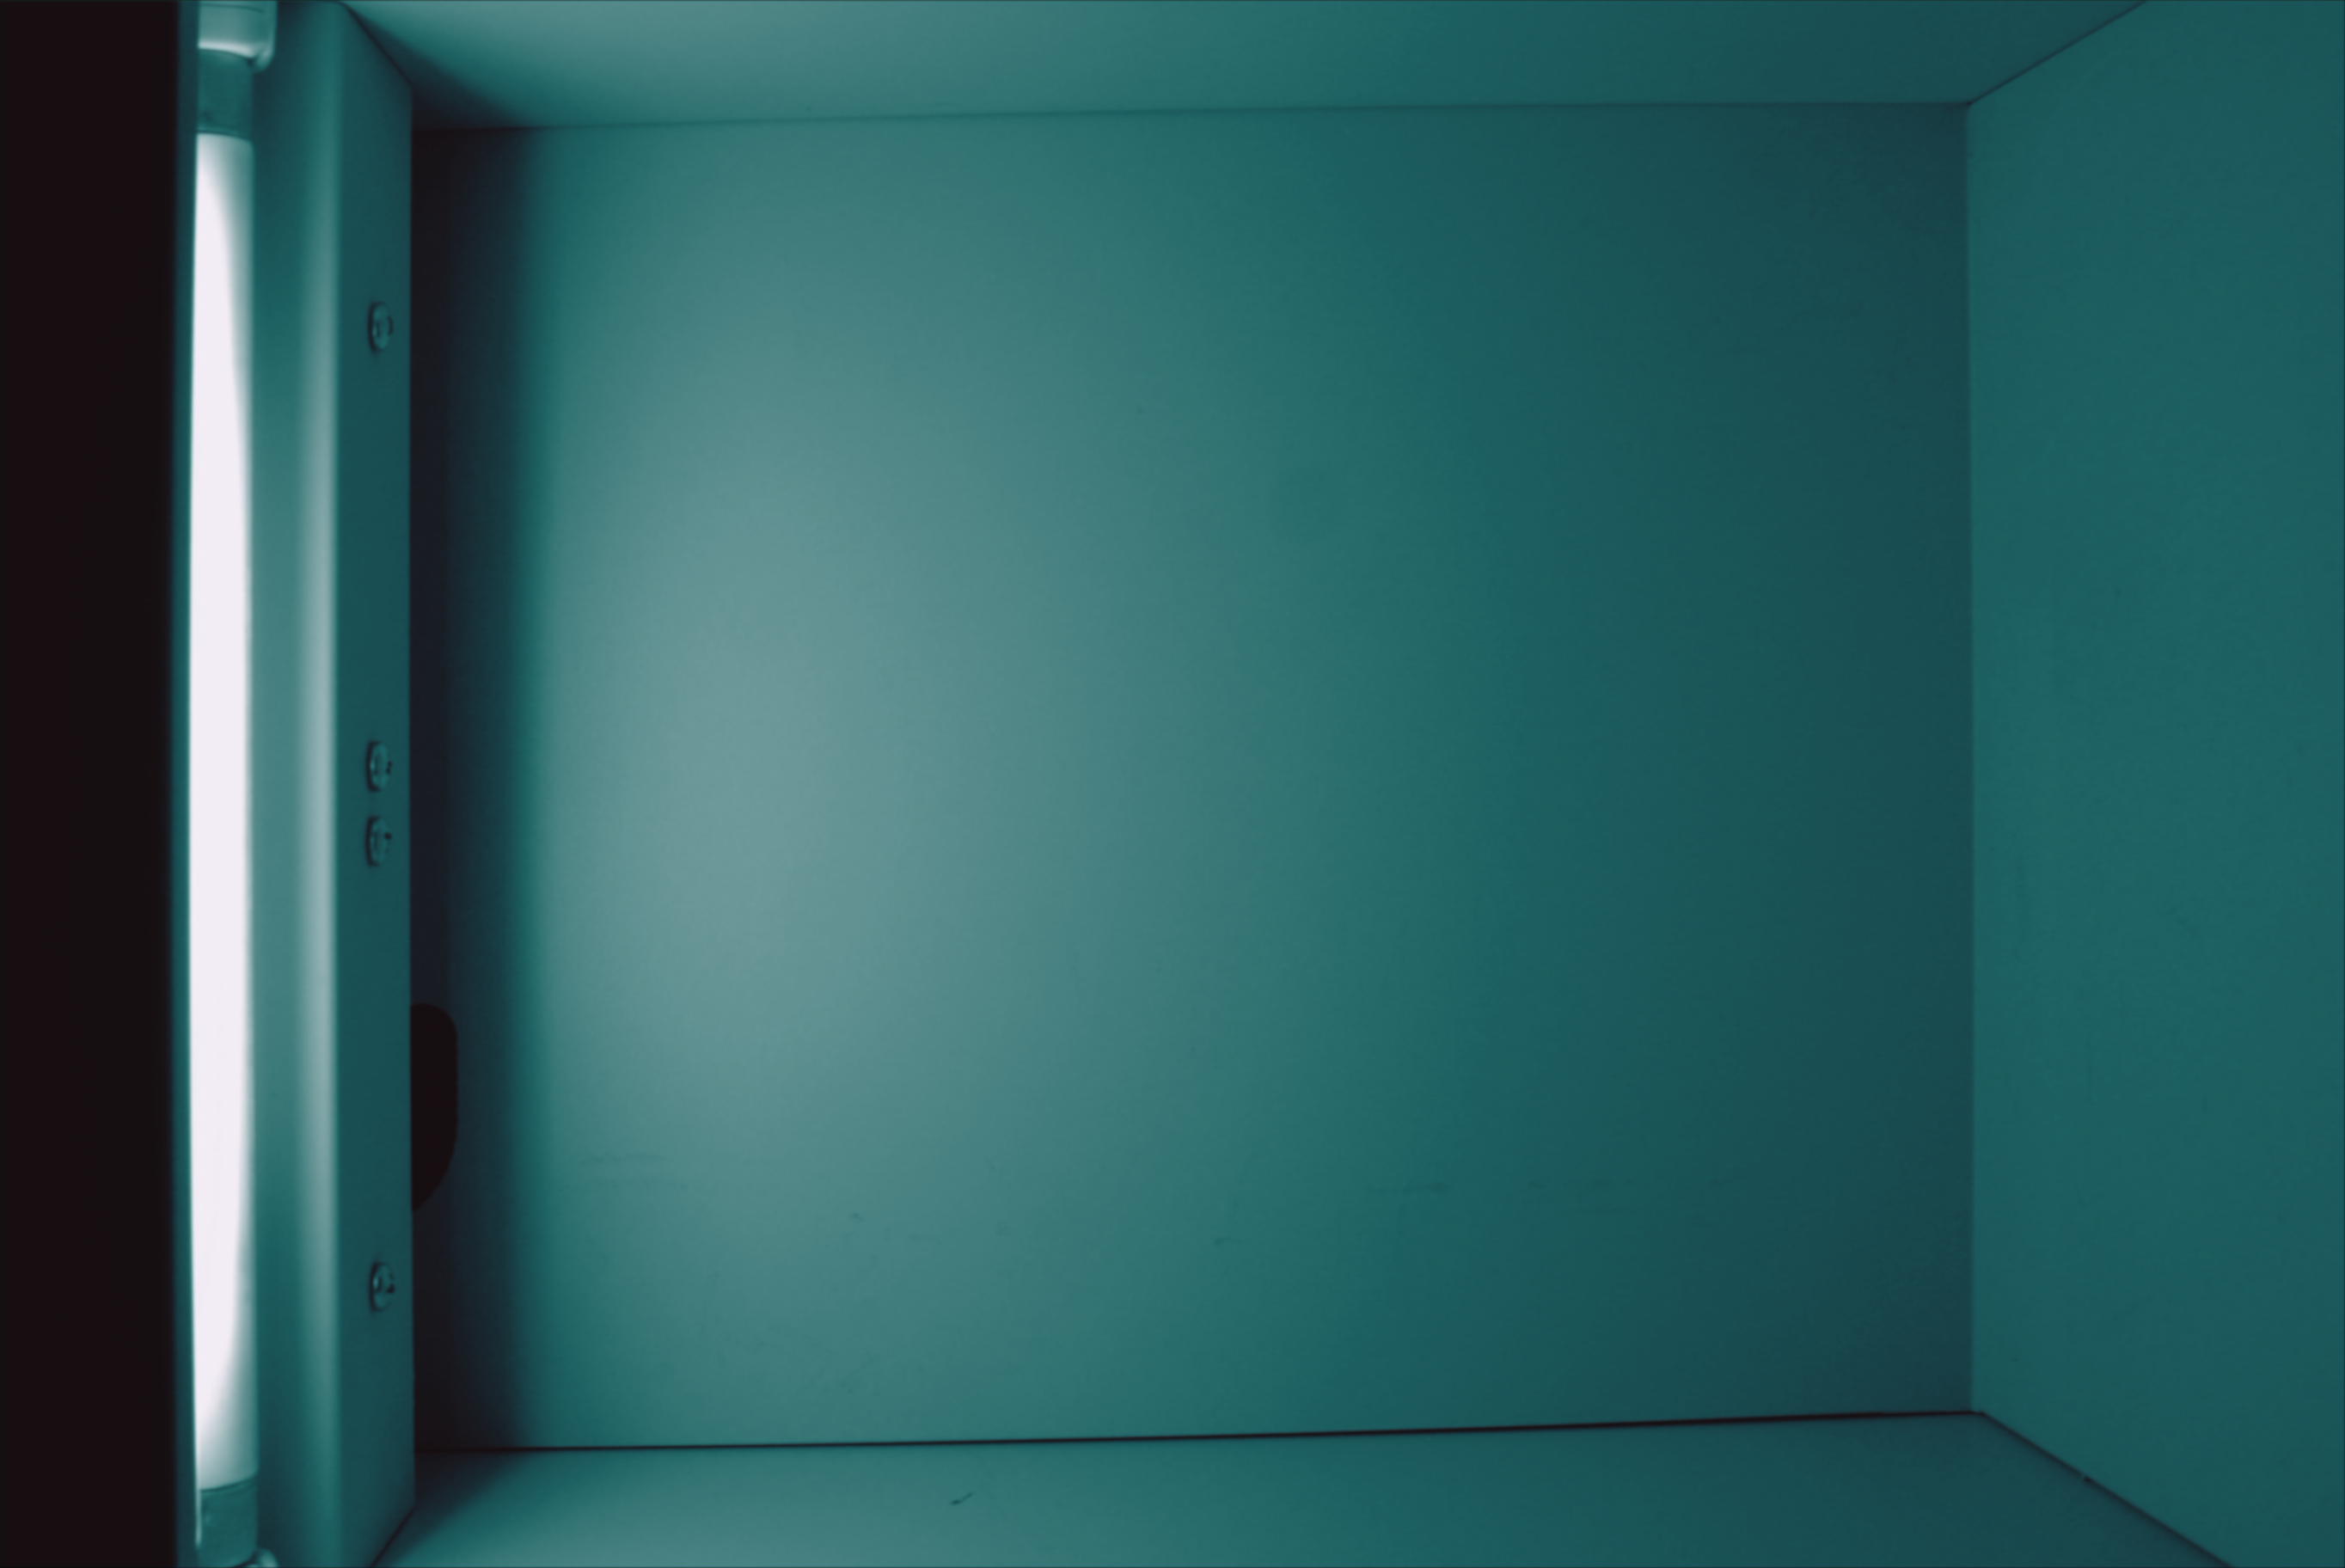
\includegraphics[width=\linewidth]{figures/mse-vgg-no-noise-resize-single.png}
        \caption{MSE/VGG \\ no noise, resize \\ LPIPS: 0.35 \\ SSIM: \textbf{0.71}}
      \end{subfigure}
    \hfill
    \begin{subfigure}[t]{.19\textwidth}
        \centering
        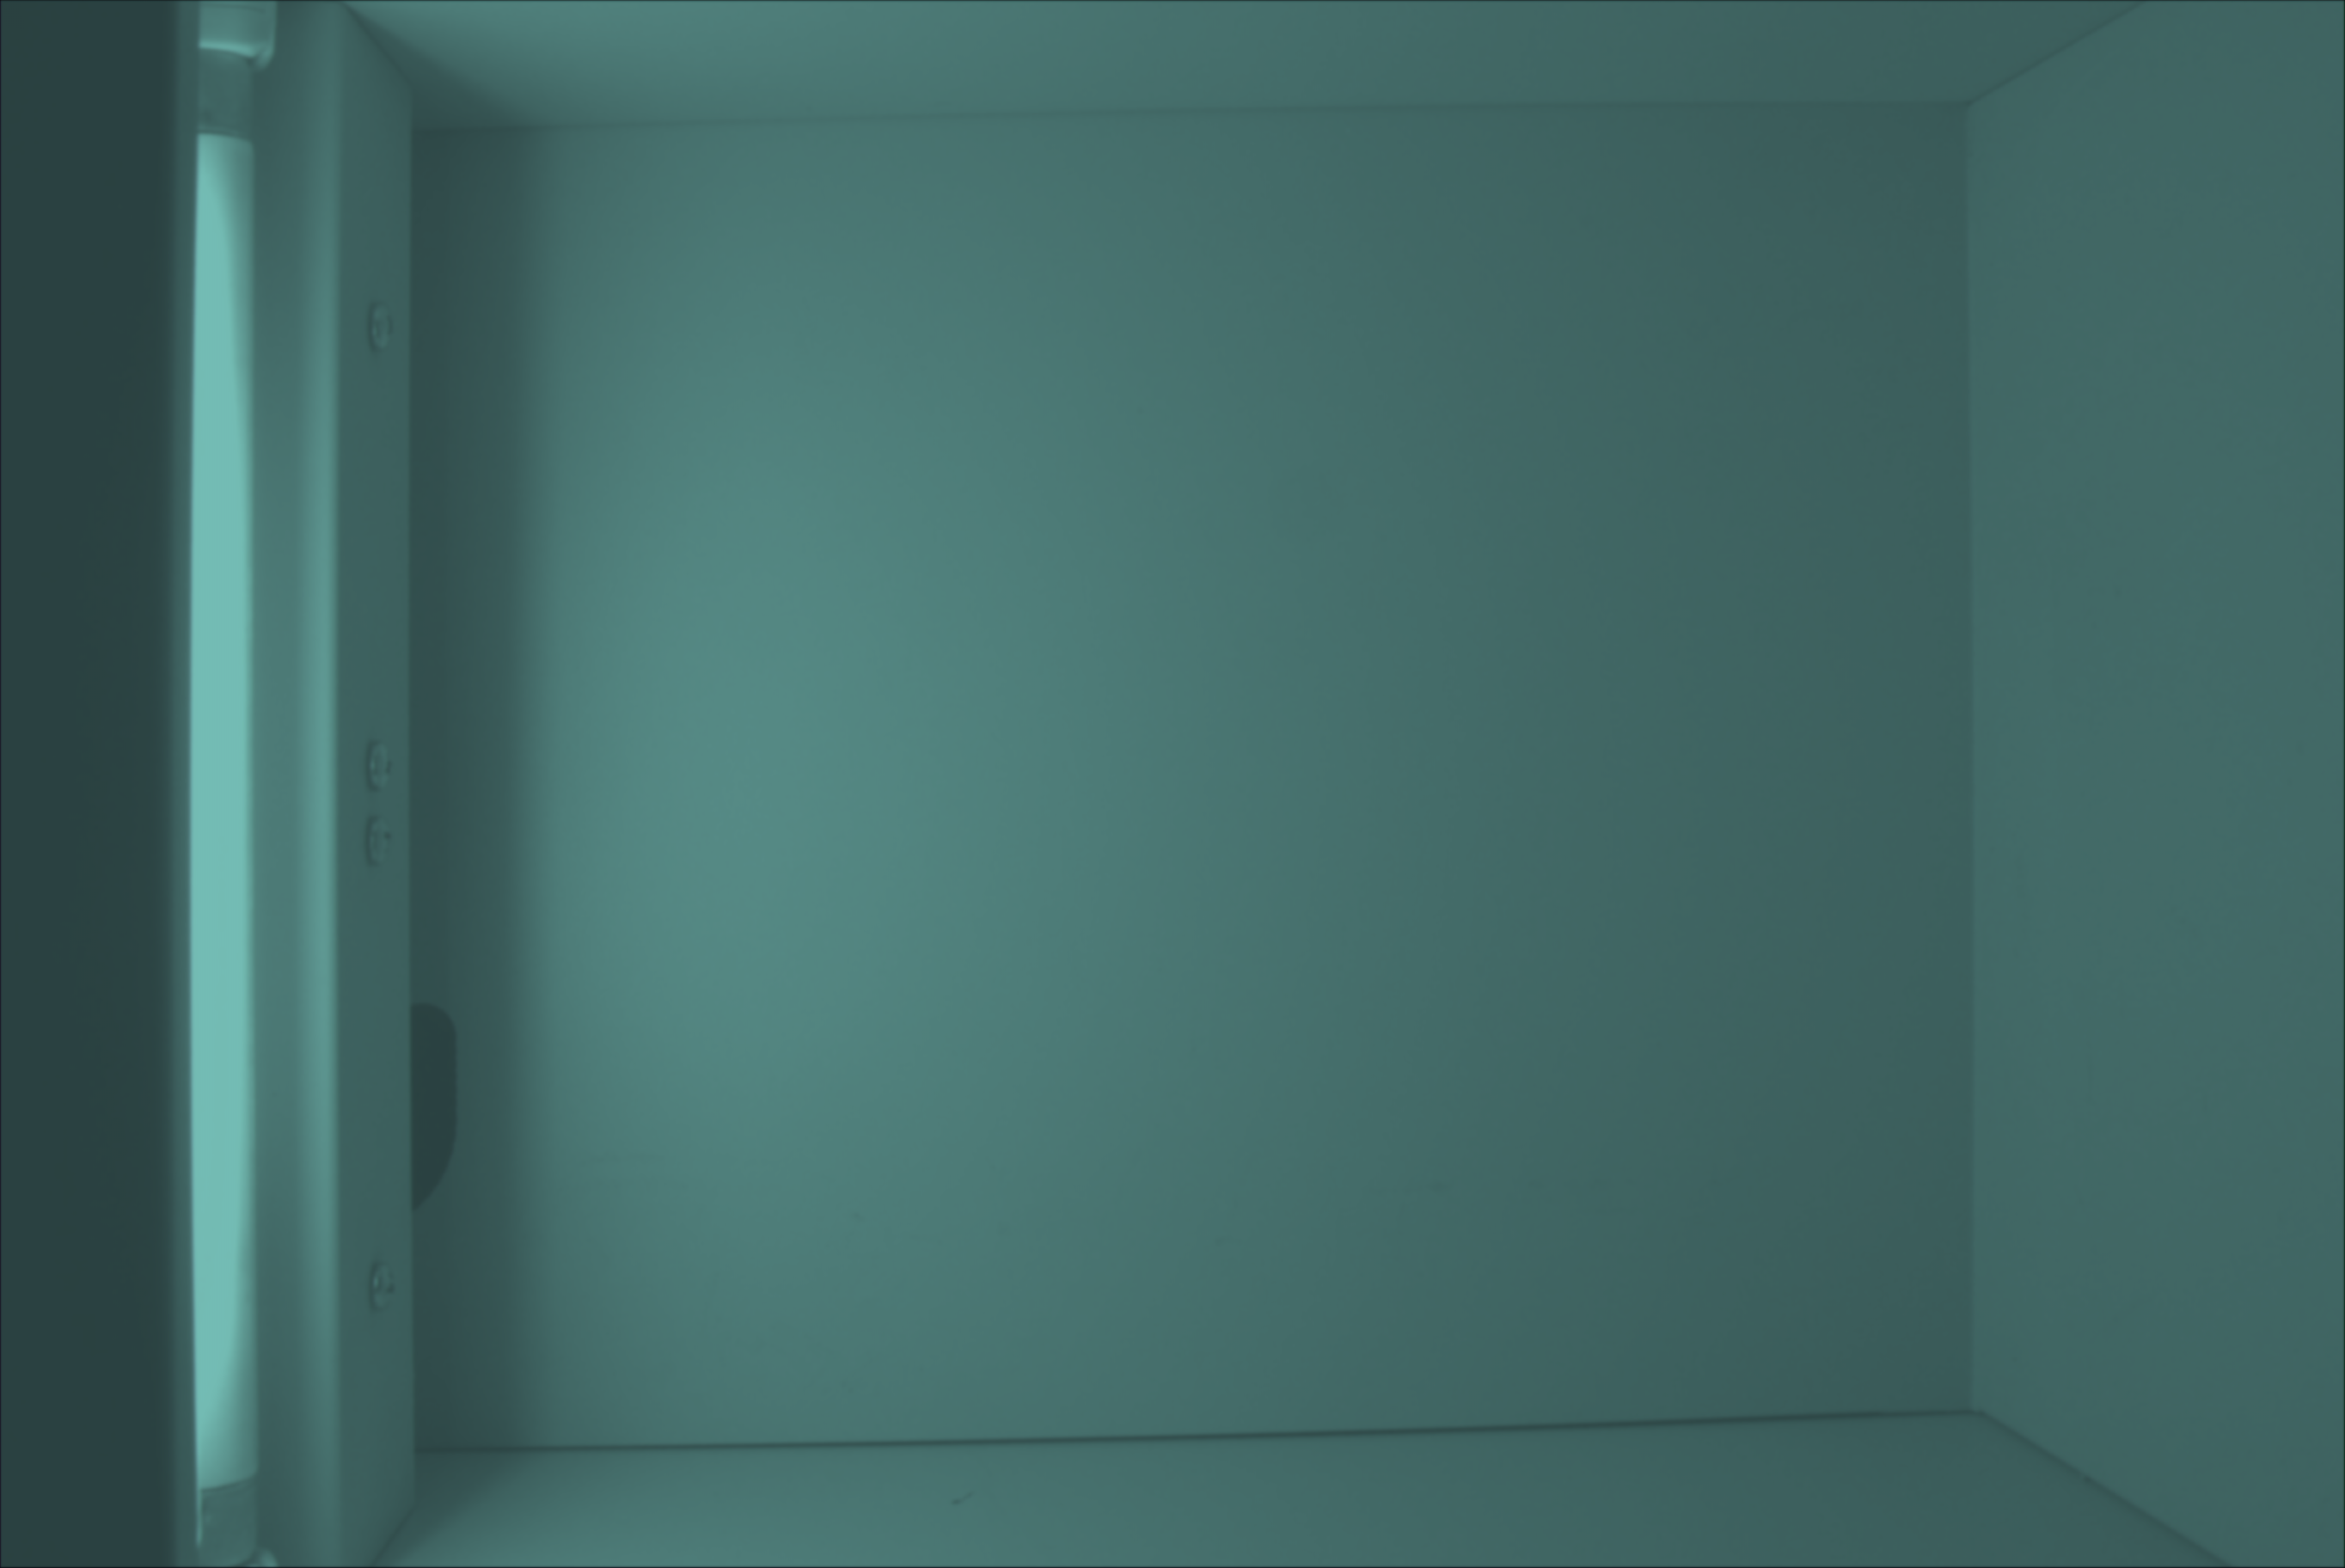
\includegraphics[width=\linewidth]{figures/mse-no-noise-no-resize-single.png}
        \caption{MSE \\ no noise, no resize \\ LPIPS: 0.47 \\ SSIM: 0.67}
      \end{subfigure}
    \hfill
    \begin{subfigure}[t]{.19\textwidth}
      \centering
      \includegraphics[width=\linewidth]{figures/tv-rel-single.png}
        \caption{TV-Rel \\ noise, no resize \\ LPIPS: \textbf{0.27} \\ SSIM: 0.27}
    \end{subfigure}
    \hfill
    \begin{subfigure}[t]{.19\textwidth}
        \centering
        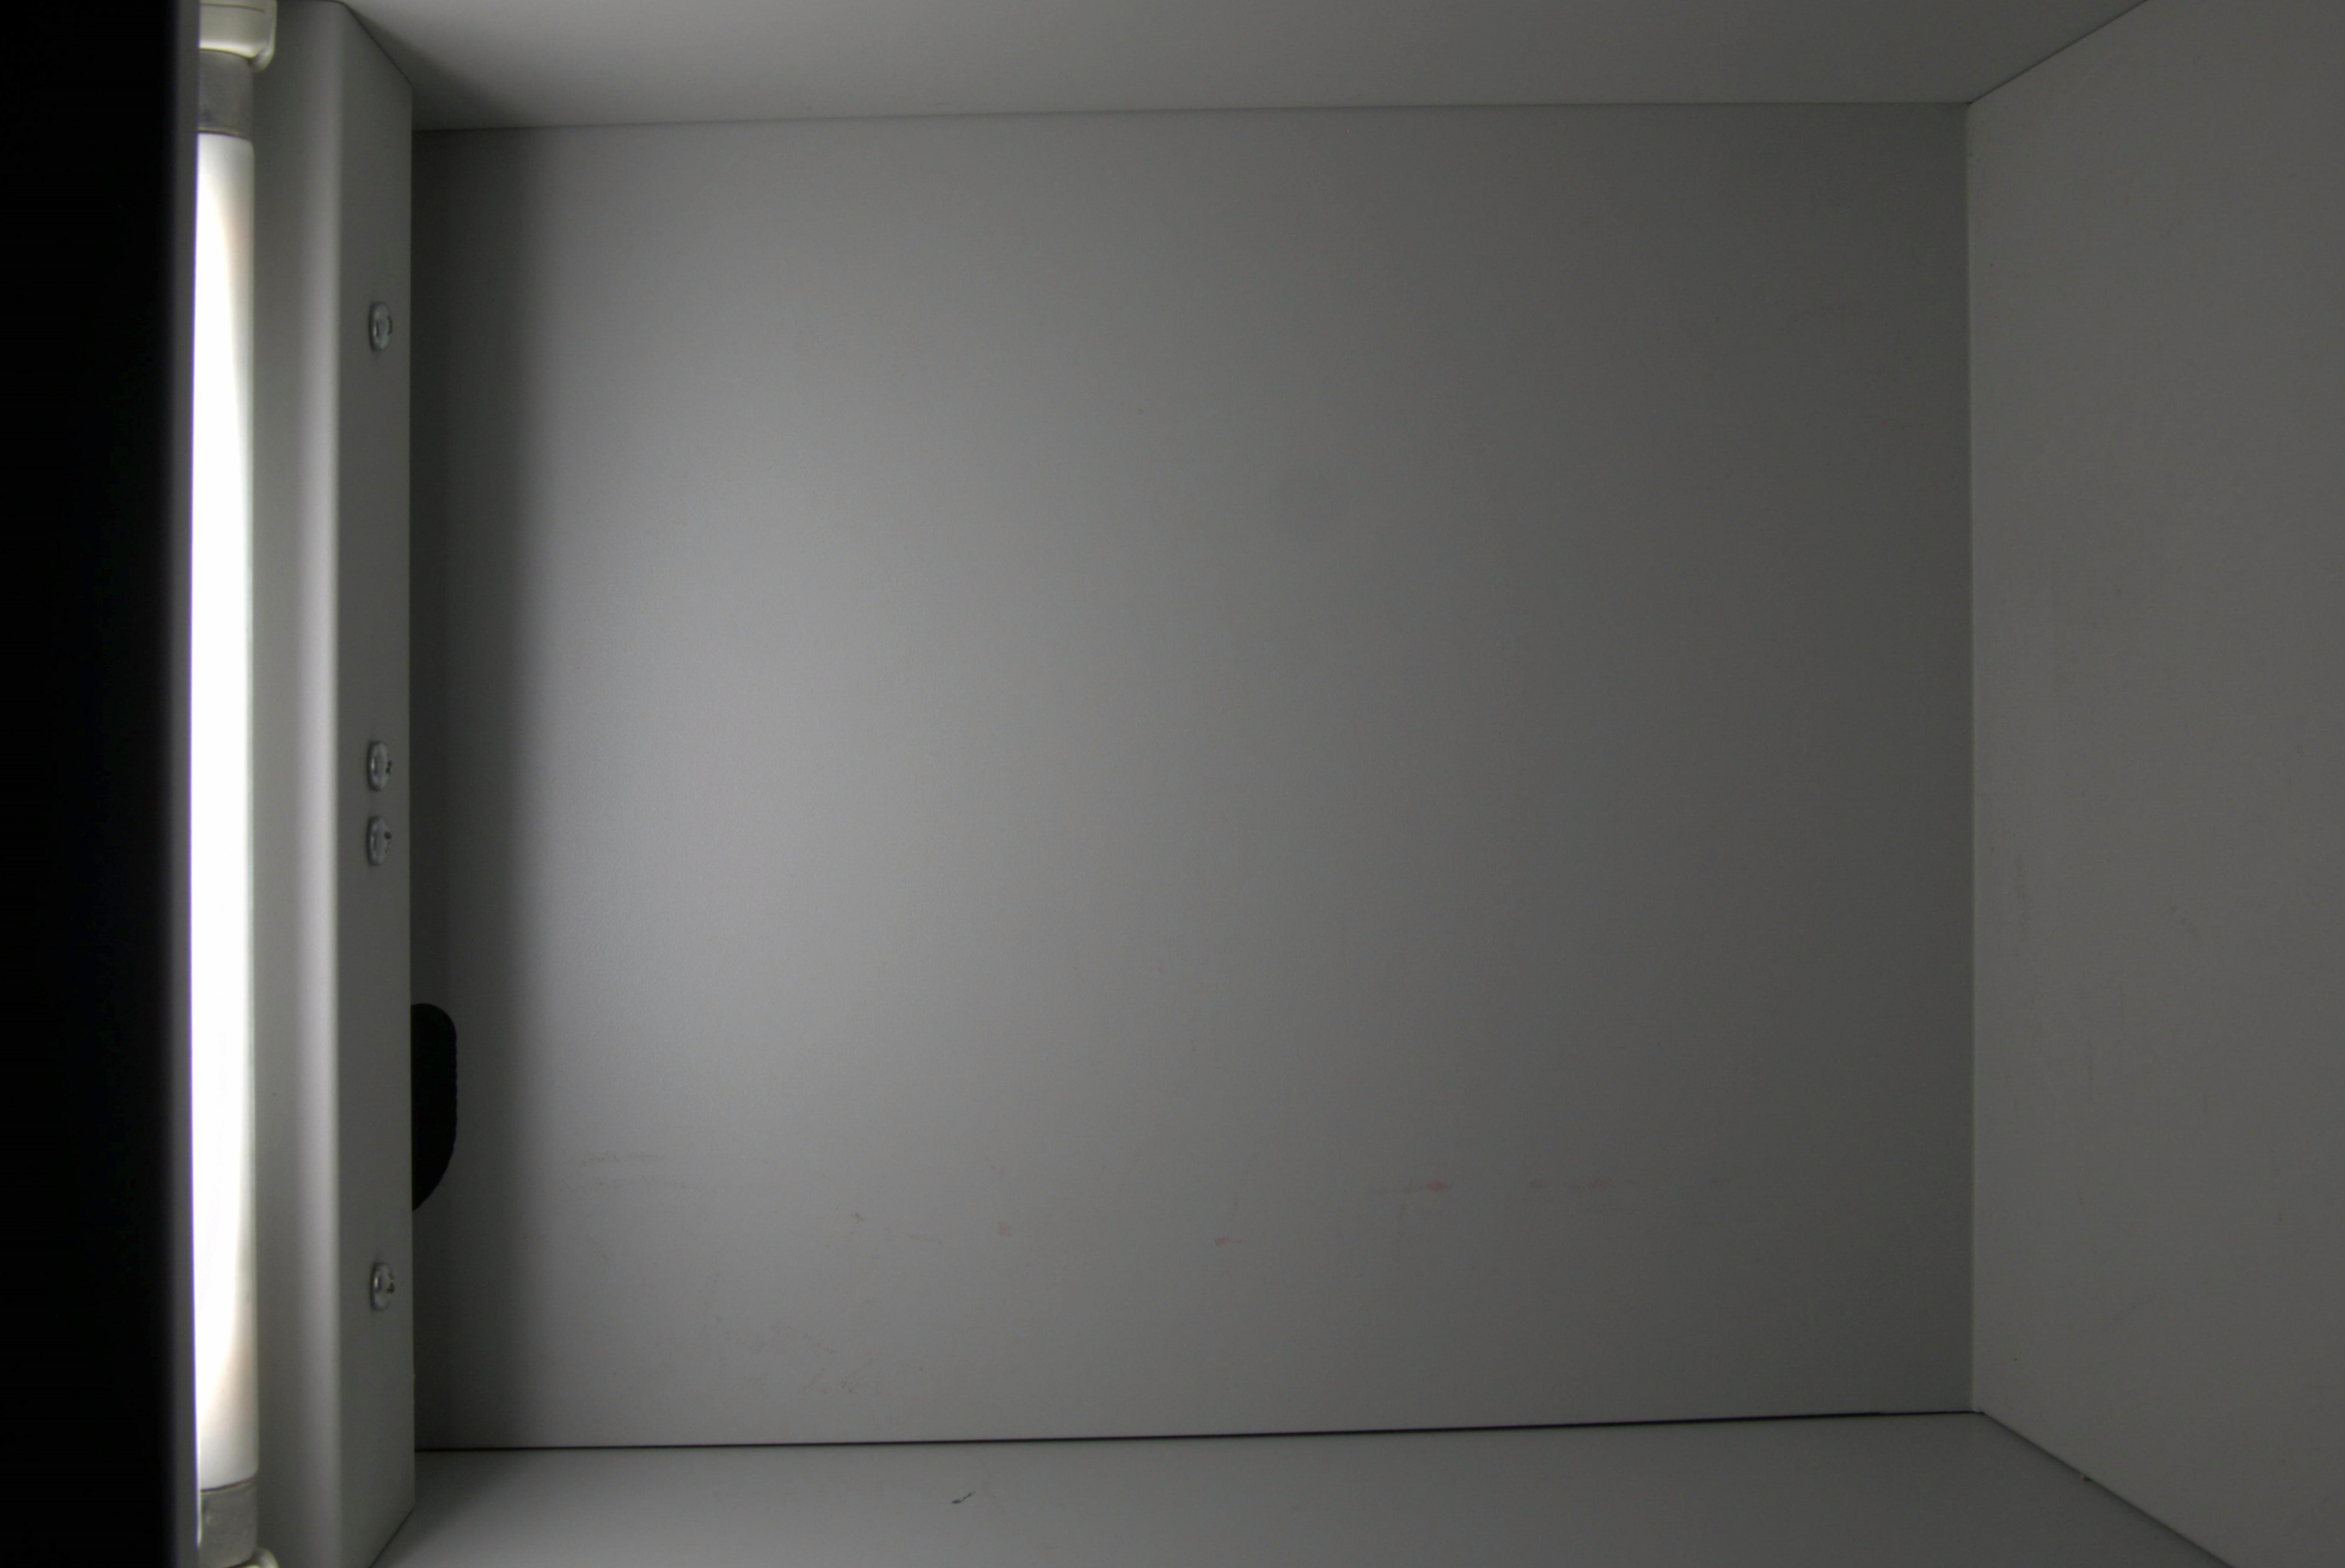
\includegraphics[width=\linewidth]{figures/digital-single.png}
        \caption{Baseline \\ \\ LPIPS: 0.36 \\ SSIM: 0.64}
      \end{subfigure}
  
    \caption{\textbf{Single Image Select Samples.} Outputs from select loss functions and configurations of noise and resizing. We see that the best performing model is MSE/VGG with resizing, which produces the best colour effect. We also see that LPIPS scores are inconsistent with SSIM and with perception as we can intuitively see that MSE-VGG and MSE are better predicitions than the baseline and TV-Rel.}

    \label{fig:single-image-samples}
\end{figure}

\begin{table}
    \centering
    \captionsetup{justification=centering}
    \caption{
        \textbf{Single Image Losses.} \\Results for each loss configuration with and without noise and no resizing.
    }
    \setlength{\tabcolsep}{0.3em}
    \begin{tabular}{l|cccc|cccc}
        \toprule
        \multicolumn{1}{c}{\textbf{Loss}}& \multicolumn{4}{c}{\textbf{Without Noise}} & \multicolumn{4}{c}{\textbf{With Noise}}\\
        \multicolumn{1}{c}{} & SSIM & PSNR & LPIPS & \multicolumn{1}{c}{PieAPP} & SSIM & PSNR & LPIPS & PieAPP \\
        \midrule
        Color/VGG/TV-Rel & \textbf{0.68} & 19.67 & 0.45 & \textbf{1.42} & 0.67 & 18.01 & 0.37 & \textbf{1.14} \\
        Color/VGG & \textbf{0.68} & \textbf{20.07} & 0.45 & 1.61 & \textbf{0.68} & 17.94 & 0.36 & 1.58 \\
        MSE/VGG & 0.66 & 18.26 & 0.48 & 2.53 & 0.67 & \textbf{19.79} & 0.34 & 2.05 \\
        MAE & 0.65 & 18.61 & 0.50 & 2.12 & \textbf{0.68} & 19.04 & 0.33 & 1.96 \\
        Color & 0.65 & 18.45 & 0.50 & 2.99 & 0.63 & 15.66 & 0.43 & 2.50 \\
        MSE & 0.65 & 18.29 & 0.50 & 2.42 & 0.67 & 19.26 & 0.32 & 1.89 \\
        Baseline & 0.64 & 16.97 & \textbf{0.36} & 3.79 & 0.64 & 16.97 & 0.36 & 3.79 \\
        \midrule
        TV-Rel & 0.17 & 9.84 & 0.60 & 4.84 & 0.27 & 11.11 & \textbf{0.27} & 2.20 \\
        VGG & 0.16 & 9.10 & 0.62 & 4.50 & 0.06 & 8.71 & 0.64 & 5.11 \\
        \bottomrule
    \end{tabular}
    
    \label{tab:single-image-losses}
\end{table}


The addition of noise has mixed effects. The perceptual metrics significantly reward the addition of noise in almost all cases. SSIM and PSNR react differently depending on the loss: pixel-wise MSE/MAE scores increase slightly, whereas Color loss scores decrease. This can be interpreted as Color loss allowing more noise through the model which is penalised by metrics sensitive to incorrect random noise such as PSNR, where MAE/MSE will even out this noise to be closer to the ground truth, on average. All of this implies that the perceptual metrics better capture the output of noise by the model. Comparisons of outputs from the models with and without noise channels can be seen in Figure \ref{fig:single-image-noise-no-noise}.

\begin{figure}

    \begin{subfigure}[t]{.24\textwidth}
        \centering
        
\includegraphics[width=\linewidth]{figures/color-vgg-tv-rel-noise-patch-single.png}
        
      \end{subfigure}
    \hfill
    \begin{subfigure}[t]{.24\textwidth}
        \centering
        
\includegraphics[width=\linewidth]{figures/mse-vgg-noise-no-resize-patch-single.png}
    \end{subfigure}
    \hfill
    \begin{subfigure}[t]{.24\textwidth}
        \centering
        
\includegraphics[width=\linewidth]{figures/mse-noise-no-resize-patch-single.png}
    \end{subfigure}
    \hfill
    \begin{subfigure}[t]{.24\textwidth}
        \centering
        
\includegraphics[width=\linewidth]{figures/film-patch-single.png}
      \end{subfigure}


    \begin{subfigure}[t]{.24\textwidth}
        \centering
        
\includegraphics[width=\linewidth]{figures/color-vgg-tv-rel-no-noise-patch-single.png}
        \captionsetup{justification=centering}
        \caption{Color/VGG/TV-Rel}
      \end{subfigure}
        \hfill
    \begin{subfigure}[t]{.24\textwidth}
        \centering
        
\includegraphics[width=\linewidth]{figures/mse-vgg-no-noise-no-resize-patch-single.png}
        \caption{\\MSE/VGG}
      \end{subfigure}
    \hfill
    \begin{subfigure}[t]{.24\textwidth}
        \centering
        
\includegraphics[width=\linewidth]{figures/mse-no-noise-no-resize-patch-single.png}
        \caption{\\MSE}
    \end{subfigure}
    \hfill
    \begin{subfigure}[t]{.24\textwidth}
        \centering
        
\includegraphics[width=\linewidth]{figures/digital-patch-single.png}
        \captionsetup{justification=centering}
        \caption{Film (Above) \\ Digital (Below)}
      \end{subfigure}
   
      \centering

    \caption{\textbf{Single Image Noise Comparison.} Outputs from select models without noise (above) and with noise (below), no resizing. We see that when we feed noise into the model, the model learns to produce some variation, especially when the loss contains a feature-based metric like VGG. However, the grain is far from the desired effect.}
    \label{fig:single-image-noise-no-noise}
\end{figure}

We also experiment with resizing cropped patches during training. This is done by taking a crop at a random scale from the image and resizing it to the patch size, $ 256 \times 256$. The results are in Table \ref{tab:single-image-resize}. We show results for only MSE and MSE/VGG as a representative example of how both pixel-wise and combined losses perform. We also experimented with a combination of noise and resizing but found that both performed better alone.  We find that we reach peak SSIM and PSNR scores when resizing the cropped patches, and perceptual metrics also improve across the board.

We hypothesise that while resizing loses high-resolution information on grain and noise patterns, the model sees a greater variety of areas of the image in a single patch and so may capture the color transformation better which is rewarded by every metric. With the MSE/VGG loss, this colour transformation is a nearly perfect overfit as the outputs in \ref{fig:single-image-resize} show. Furthermore, some grain is still produced when we feed noise into the model despite the resizing operation potentially removing grain, as can be seen in Figure \ref{fig:single-image-resize-noise}.


\begin{figure}[ht]
    \centering

    \begin{subfigure}[b]{0.49\textwidth}
        \centering
        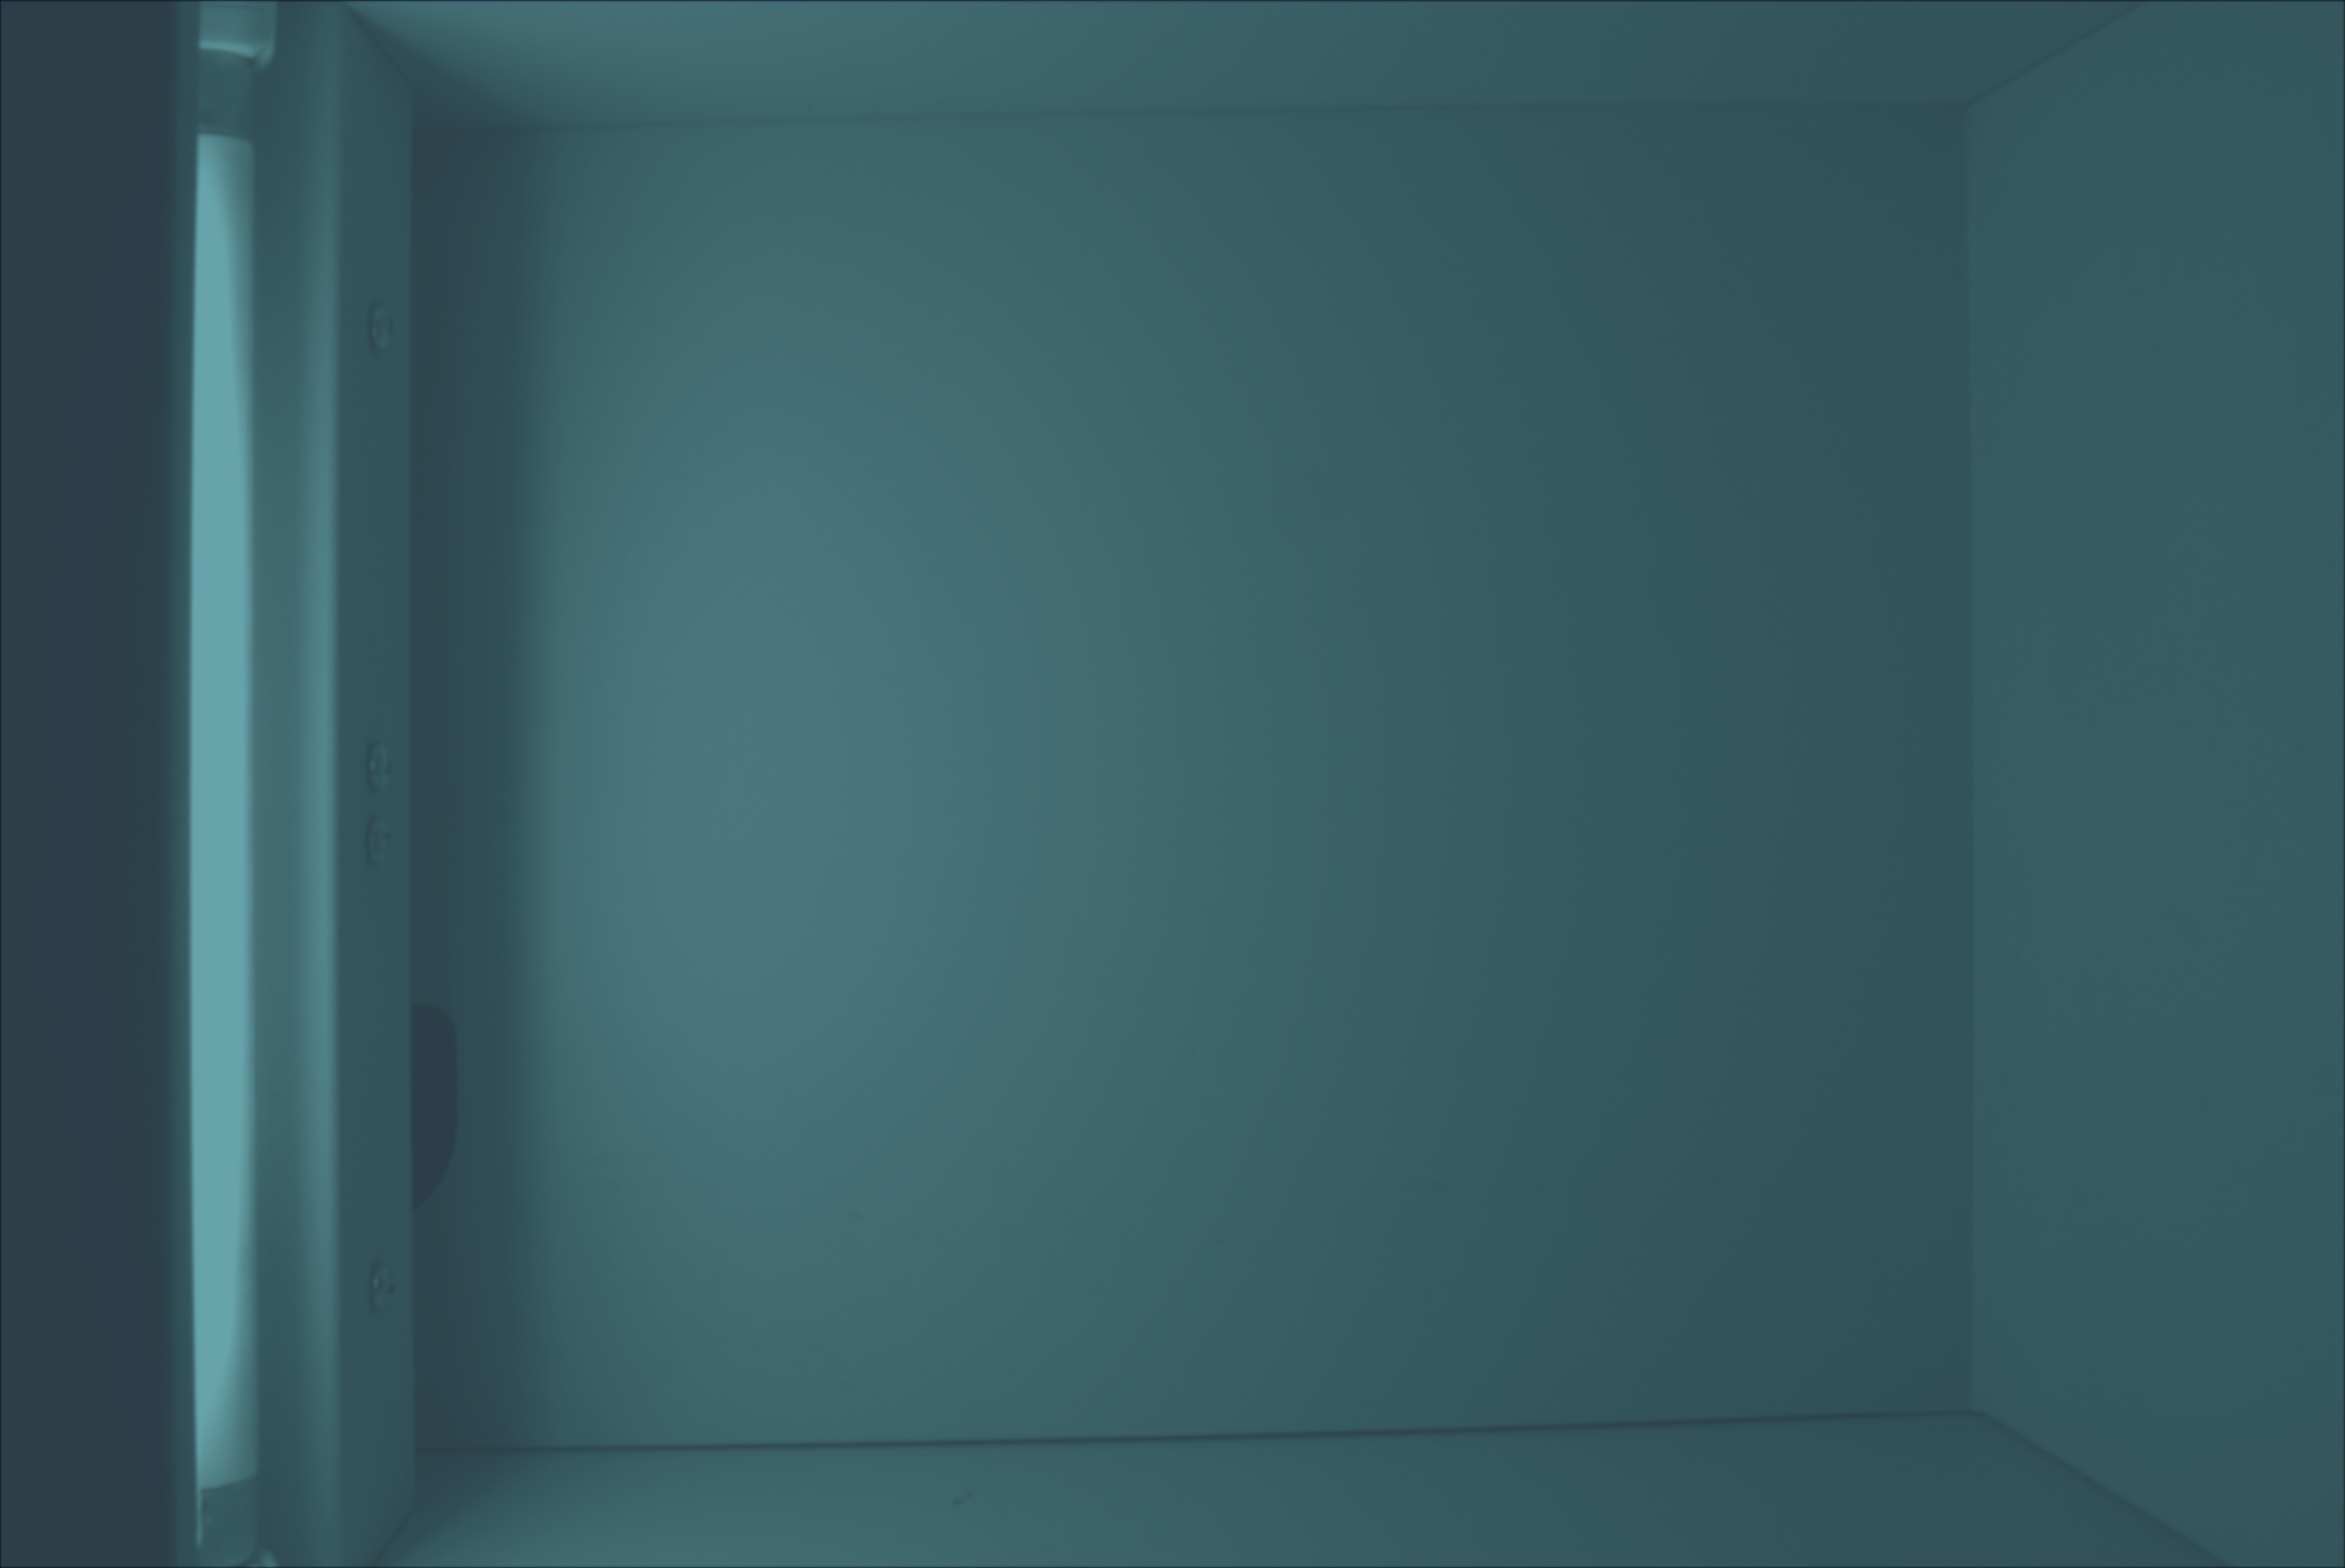
\includegraphics[width=0.49\textwidth]{figures/mse-vgg-no-noise-no-resize-single.png}
        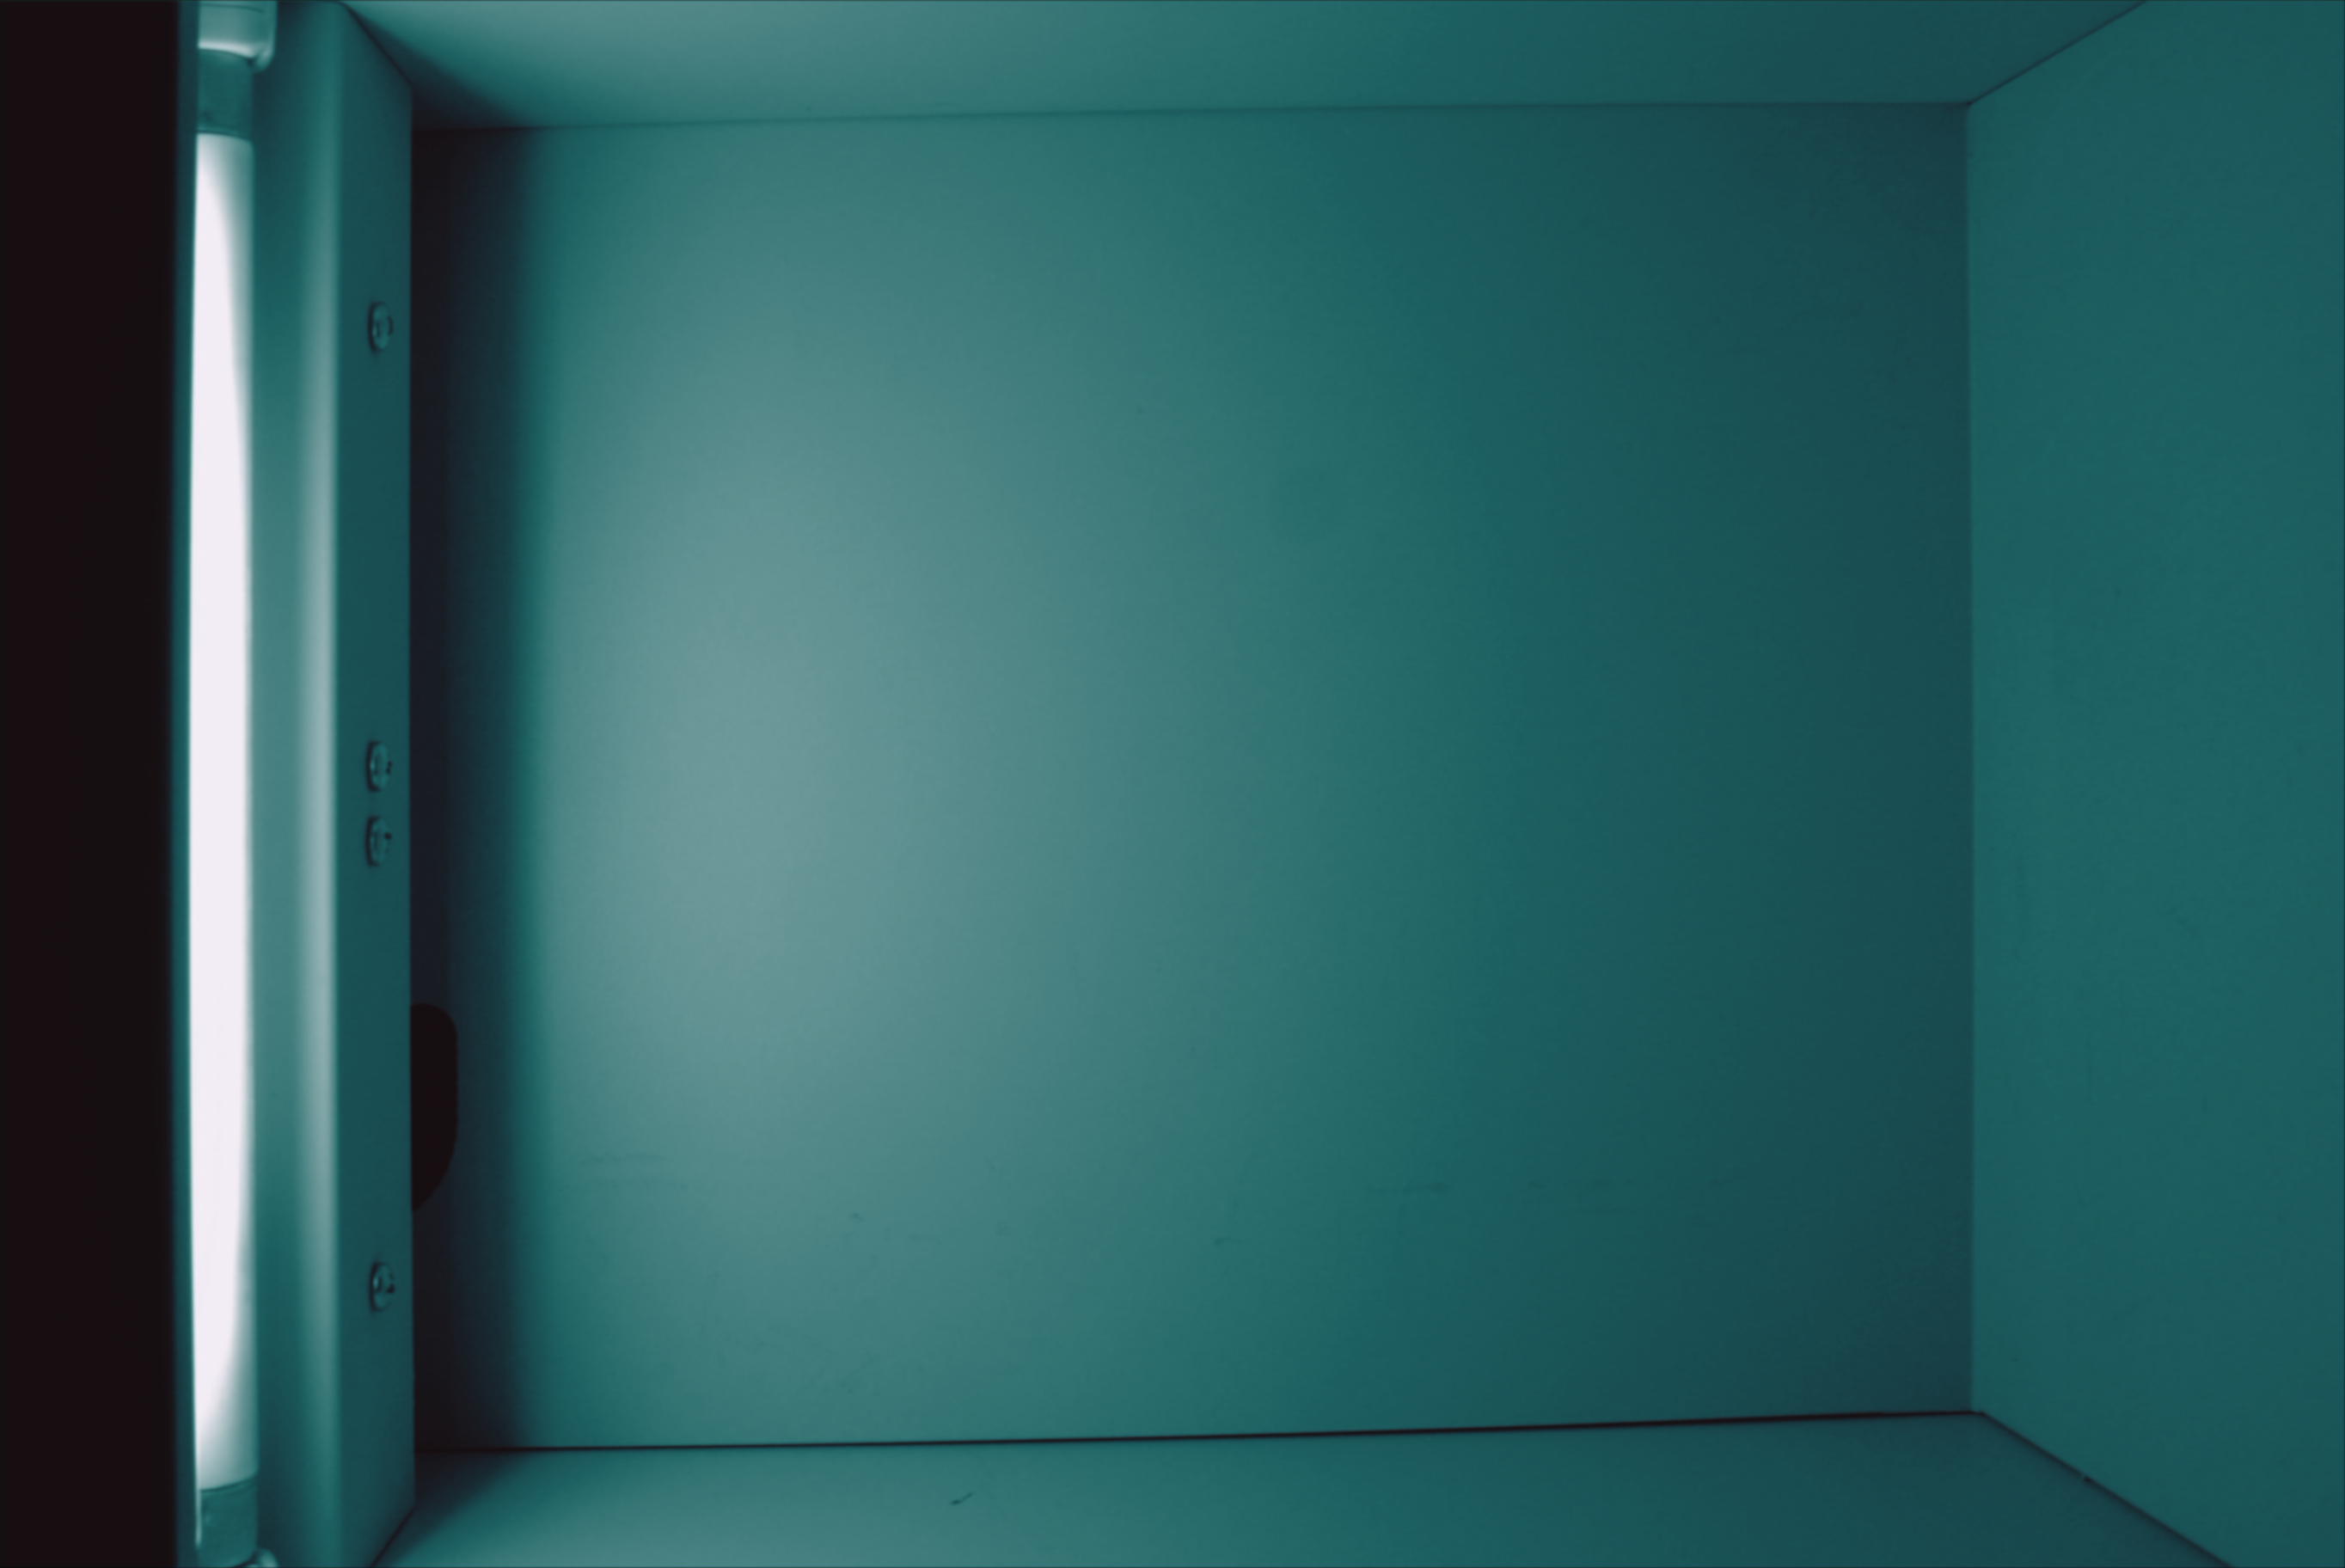
\includegraphics[width=0.49\textwidth]{figures/mse-vgg-no-noise-resize-single.png}
        \captionsetup{justification=centering}
        \caption{MSE/VGG, no noise \\ no resize (left) and with resizing (right).}
    \end{subfigure}
    \hfill
    \begin{subfigure}[b]{0.49\textwidth}
        \centering
        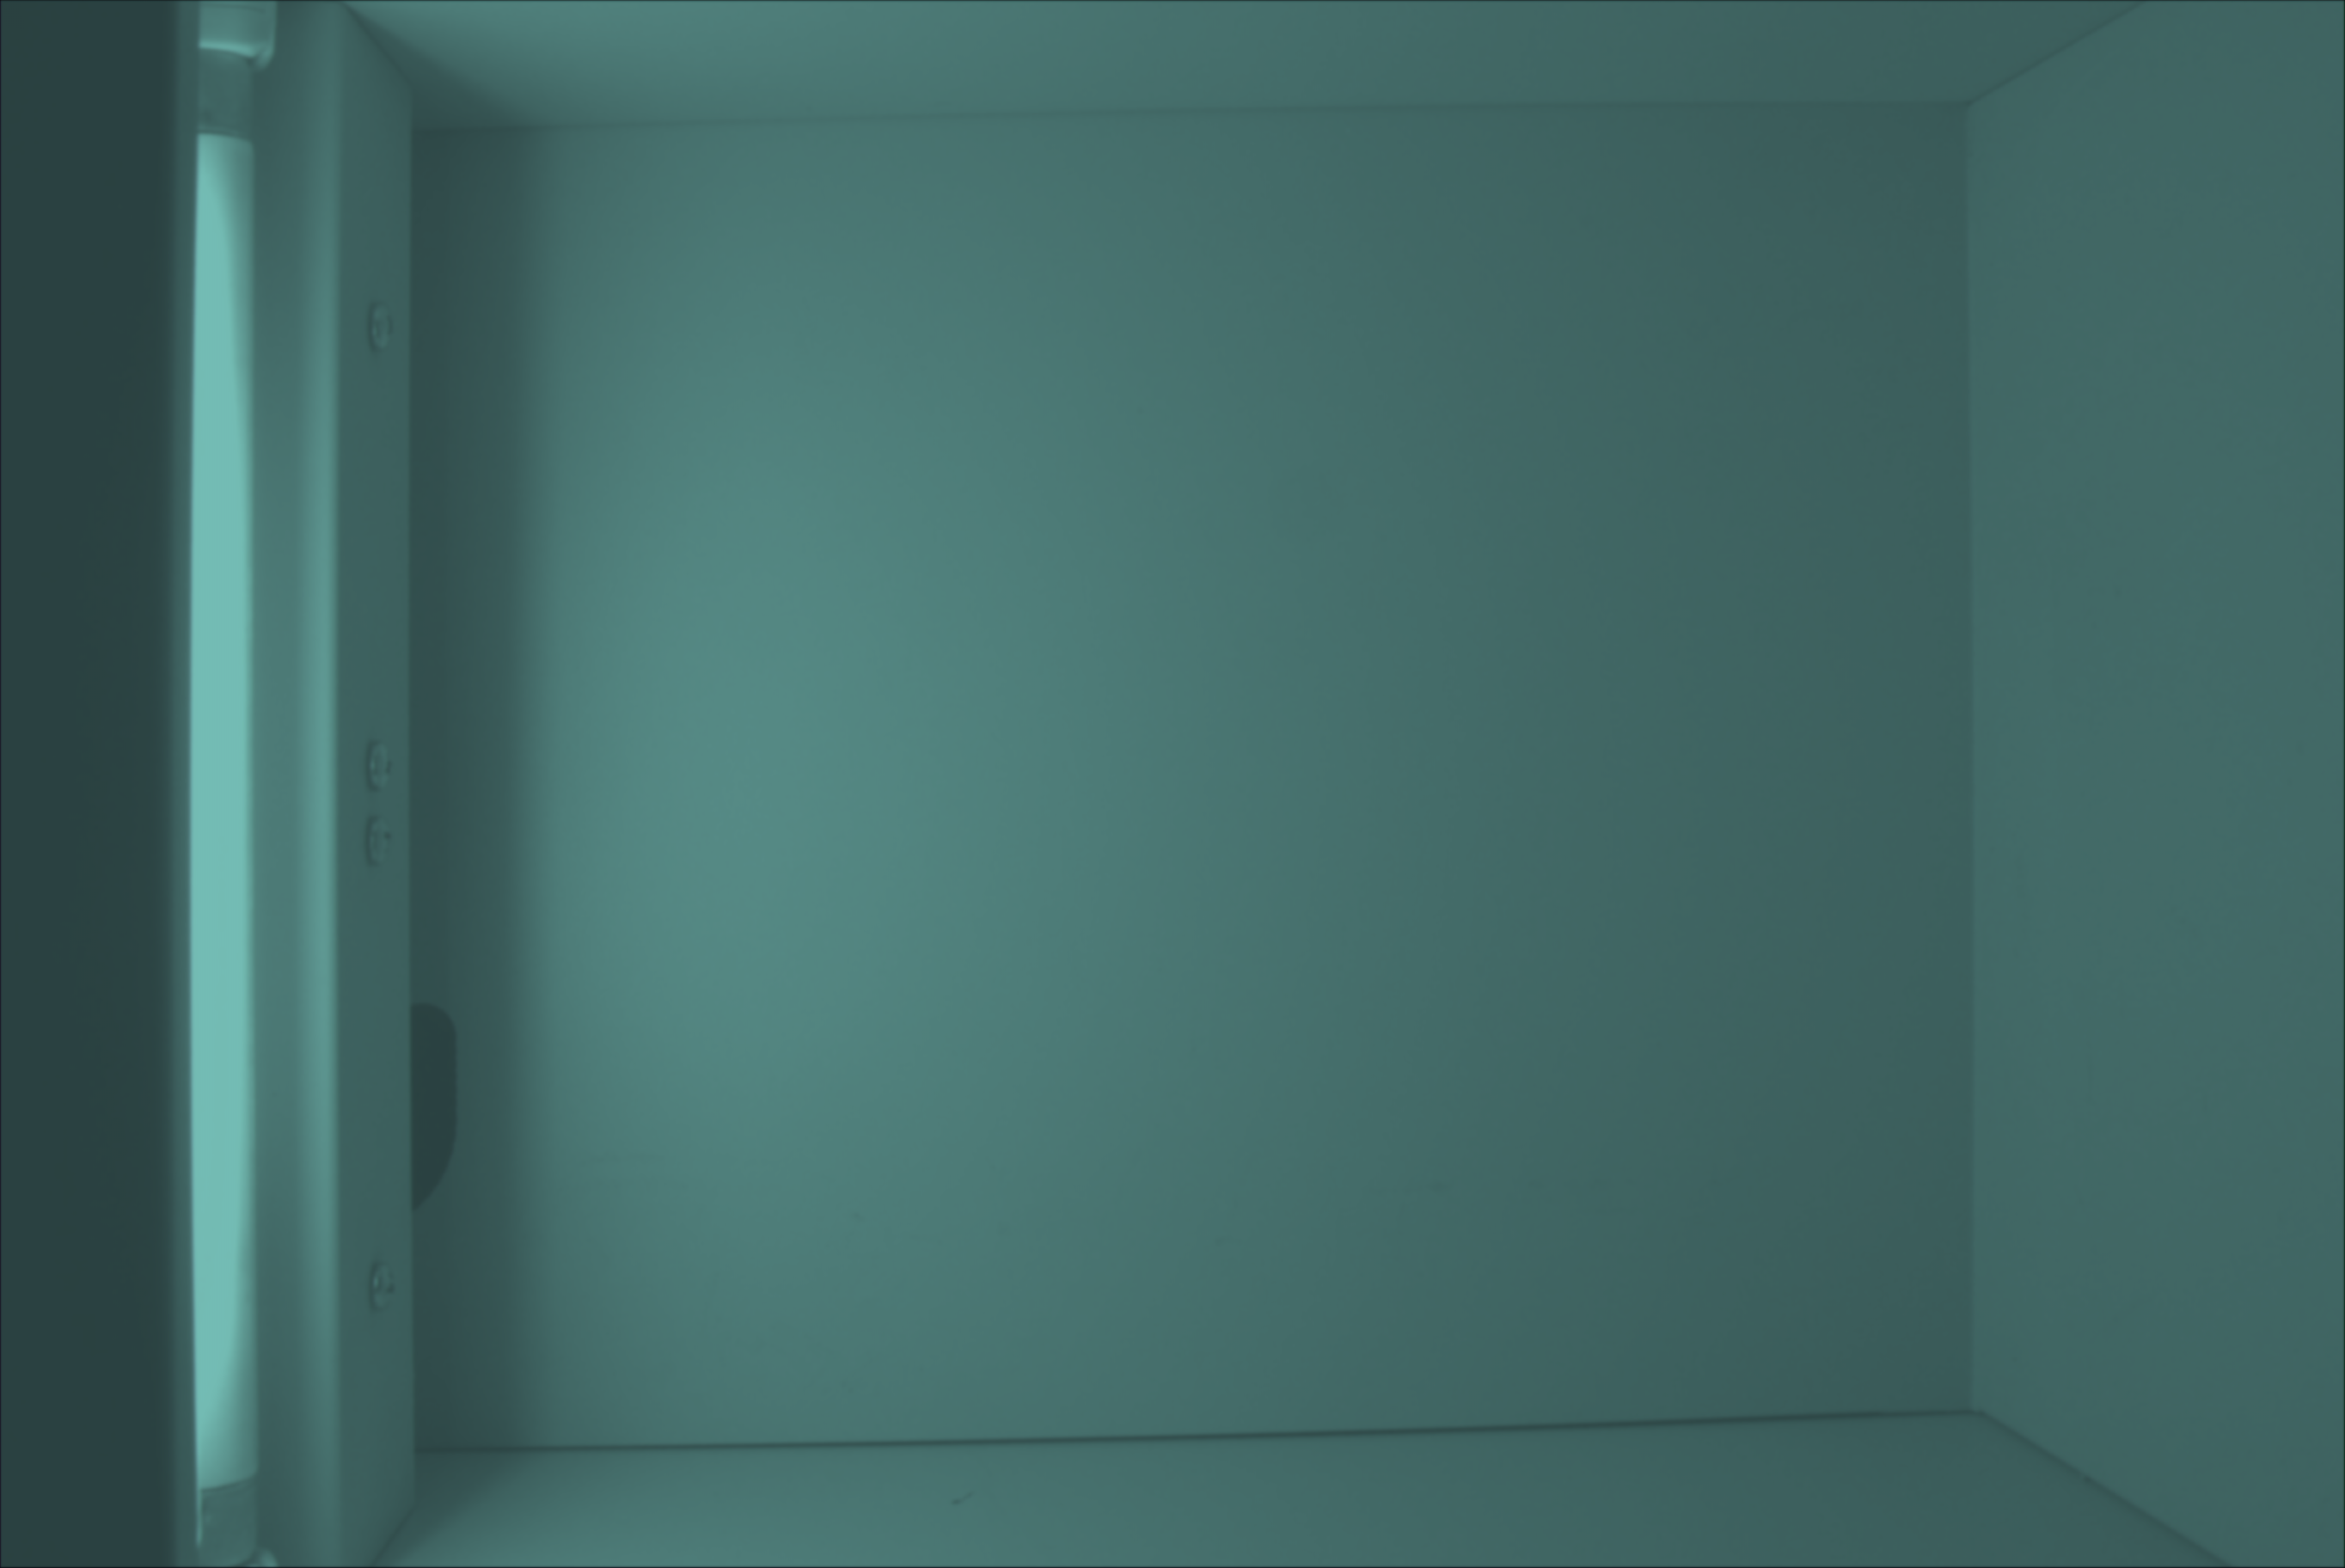
\includegraphics[width=0.49\textwidth]{figures/mse-no-noise-no-resize-single.png}
        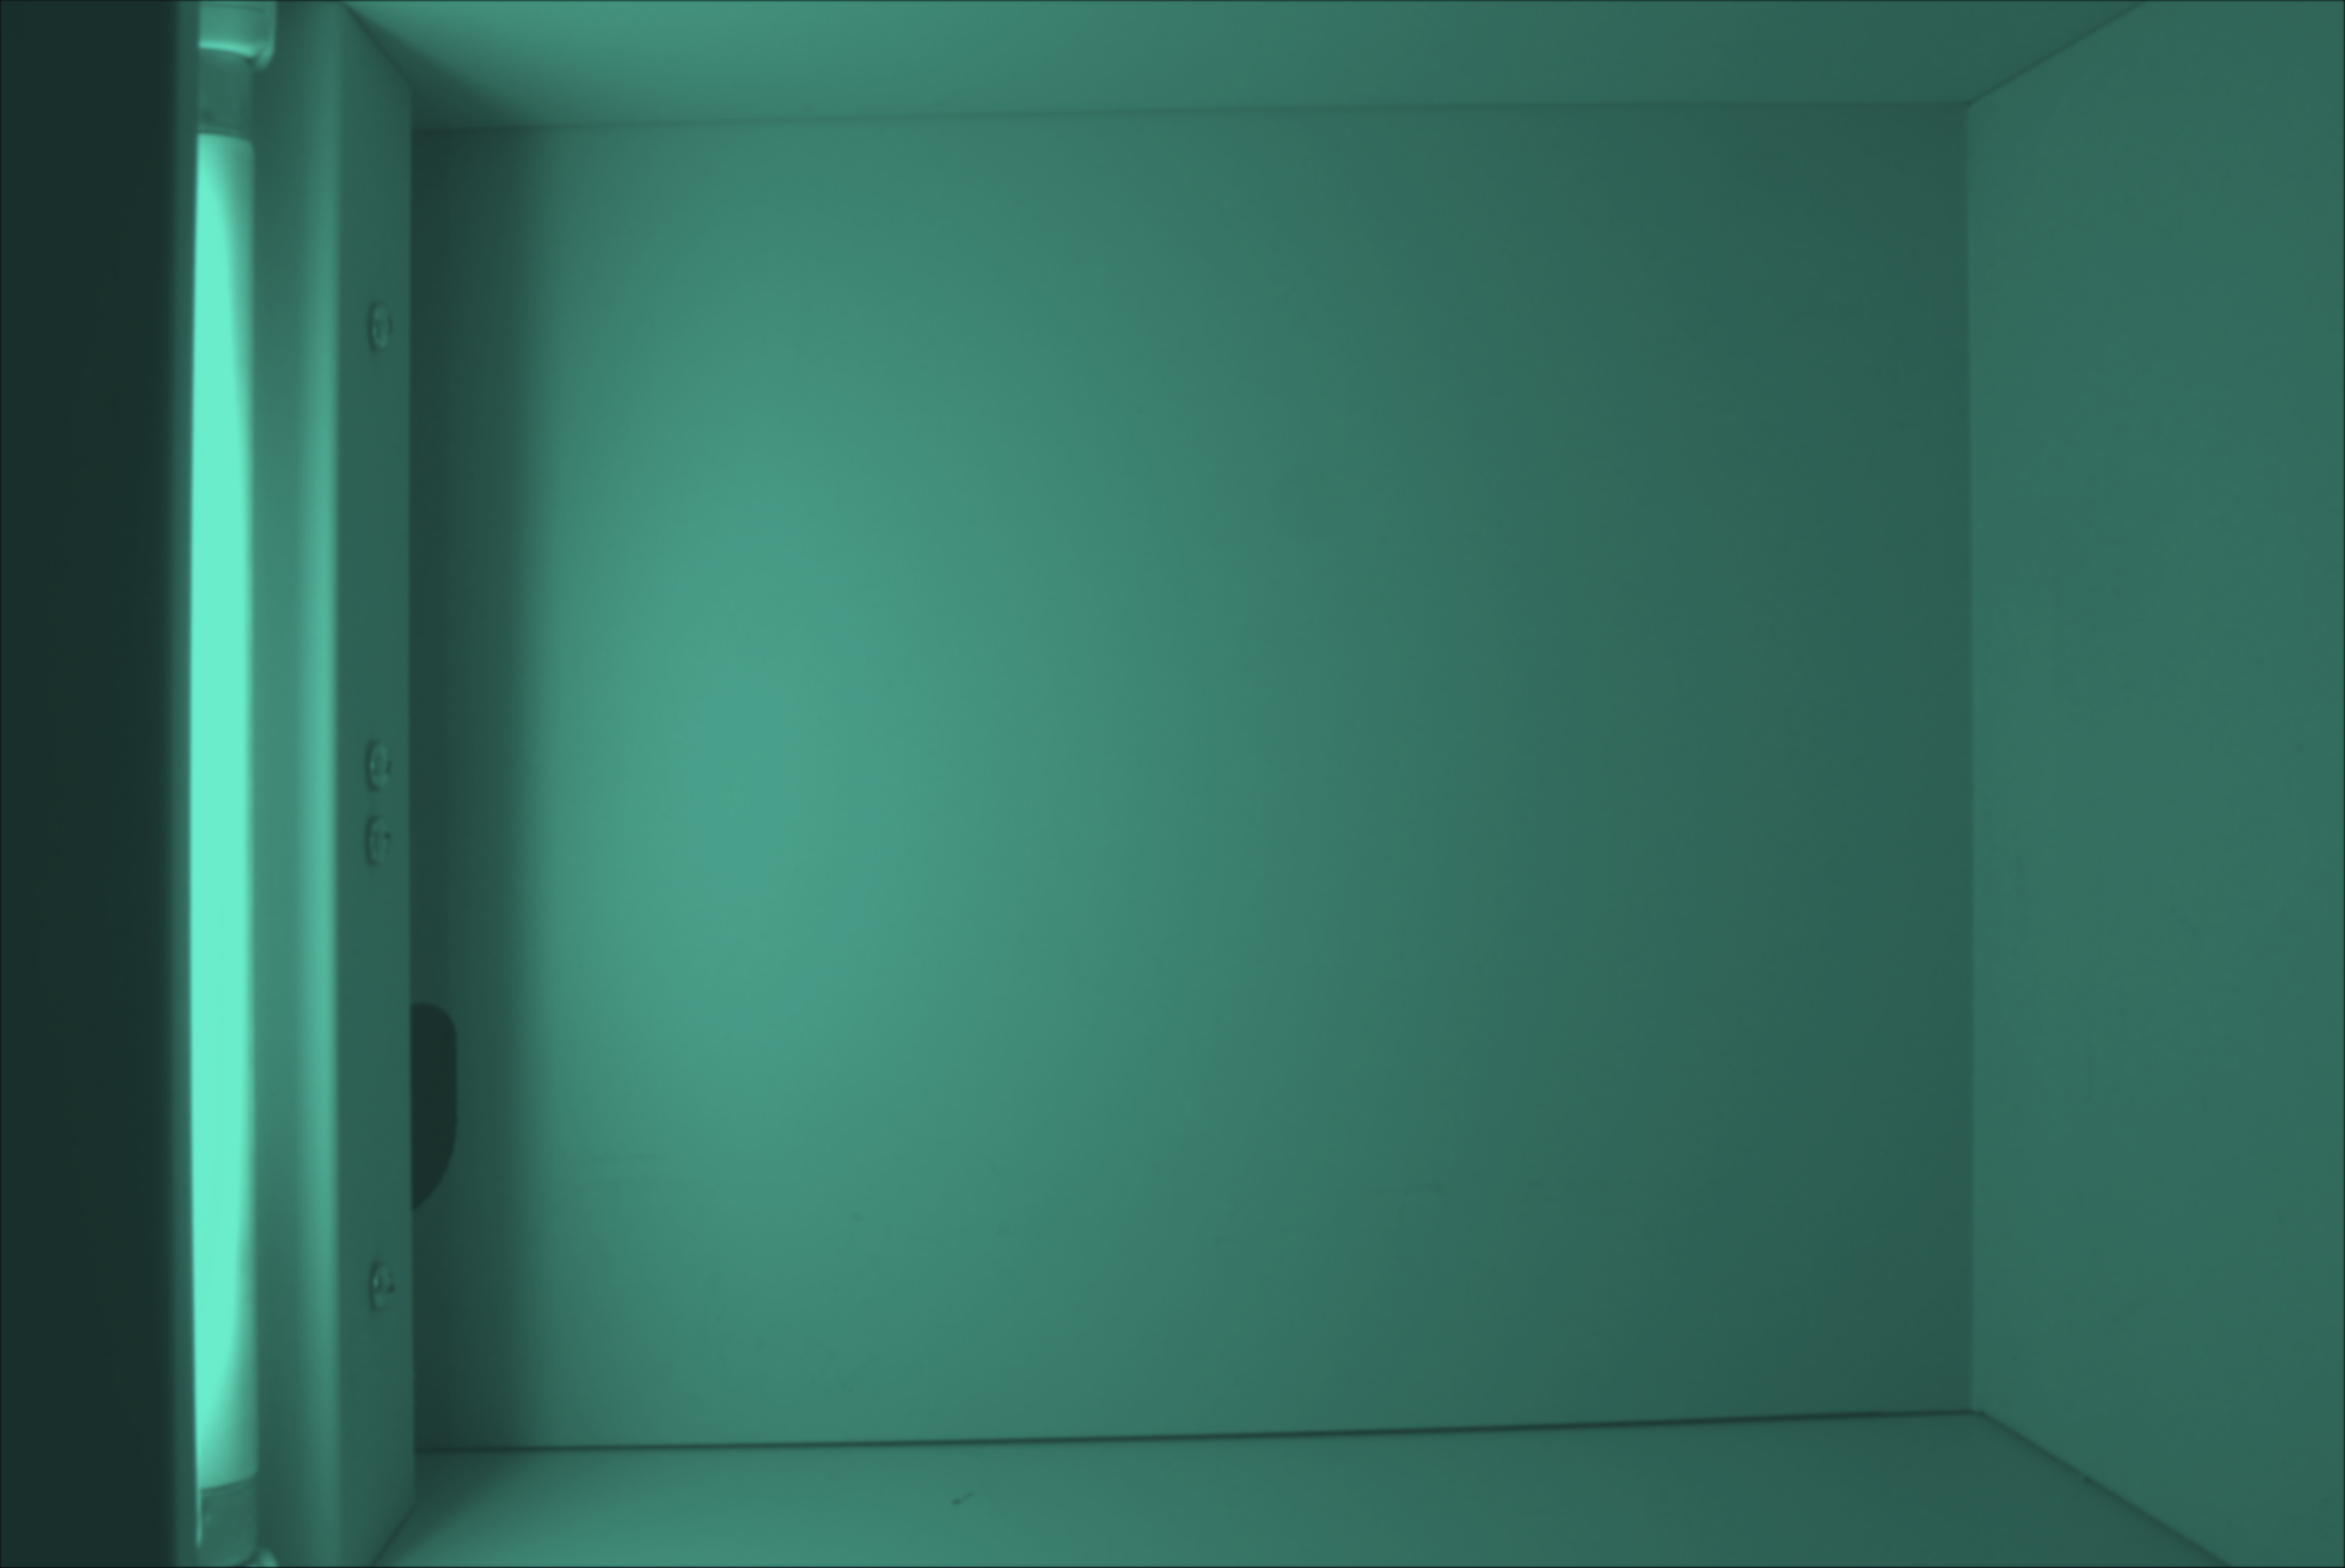
\includegraphics[width=0.49\textwidth]{figures/mse-no-noise-resize-single.png}
        \captionsetup{justification=centering}
        \caption{MSE, no noise \\ no resize (left) and with resizing (right).} 
    \end{subfigure}
    \caption{\textbf{Single Image Resizing.} Outputs from MSE and MSE/VGG with and without resizing, and then with resizing and with and without noise. We see that resizing improves the colour effect, but the grain effect is not as strong as in the single image experiments.}
    \label{fig:single-image-resize}
\end{figure}
\begin{figure}[ht]
    \begin{subfigure}[b]{0.49\textwidth}
        \centering
        
\includegraphics[width=0.49\textwidth]{figures/mse-vgg-no-noise-resize-patch-single.png}
        
\includegraphics[width=0.49\textwidth]{figures/mse-vgg-noise-resize-patch-single.png}
        \captionsetup{justification=centering}
        \caption{MSE/VGG patch with resizing \\ no noise (left) and with noise (right).} 
    \end{subfigure}
    \hfill
    \begin{subfigure}[b]{0.49\textwidth}
        \centering
        
\includegraphics[width=0.49\textwidth]{figures/mse-no-noise-resize-patch-single.png}
        
\includegraphics[width=0.49\textwidth]{figures/mse-noise-resize-patch-single.png}
        \captionsetup{justification=centering}
        \caption{MSE patch with resizing \\ no noise (left) and with noise (right).}
    \end{subfigure}

    \caption{\textbf{Single Image Resizing with Noise.} Outputs from MSE and MSE/VGG with and without noise and resizing. We see that similar grain is still produced even through resizing.}
    \label{fig:single-image-resize-noise}
\end{figure}

\begin{table}
    \centering
    \captionsetup{justification=centering}
    \setlength{\tabcolsep}{0.5em}
    \caption{
        \textbf{Single Image Resizing.} \\ Effect of resizing the cropped patches on select losses (no noise).
    }
    \begin{tabular}{lccccc}
        \toprule
        \multicolumn{1}{c}{Loss}& \multicolumn{1}{c}{Resize}&  SSIM & PSNR & LPIPS & PieAPP\\
        \midrule
        MSE/VGG & Yes & \textbf{0.71} & \textbf{23.19} & \textbf{0.35} & \textbf{1.62} \\
        MSE/VGG & No & 0.66 & 18.26 & 0.48 & 2.53 \\
        \midrule
        MSE & Yes & \textbf{0.67} & \textbf{20.03} & \textbf{0.47} & \textbf{1.77} \\
        MSE & No & 0.65 & 18.29 & 0.50 & 2.42 \\

        \bottomrule
    \end{tabular}
    
    \label{tab:single-image-resize}
\end{table}


\subsection{Full Dataset Results}

We select the best performing losses and settings from the single image experiments and evaluate them on the full dataset, with results in Table \ref{tab:full-data-results}.

\begin{table}
    \centering
    \captionsetup{justification=centering}
    \caption{\textbf{Full Dataset Results.} \\ Comparison of best performing losses and configurations on the full dataset.}
    \setlength{\tabcolsep}{0.3em}
    \begin{tabular}{lcccccc}
        \toprule
        Loss & Noise & Resize & SSIM & PSNR & LPIPS & PieAPP \\
        \midrule
        Baseline & - & - & \textbf{0.64} & 21.68 & \textbf{0.26} & 1.96 \\
        MSE/VGG & Yes & Yes & \textbf{0.64} & \textbf{22.87} & 0.27 & \textbf{1.90} \\
        MSE & No & Yes & 0.63 & 22.20 & 0.35 & 2.31 \\
        MAE & No & No & 0.59 & 19.68 & 0.48 & 3.38 \\
        Color/VGG/TV-Rel & Yes & No & 0.59 & 21.42 & 0.41 & 3.07 \\
        MSE/VGG/TV-Rel & Yes & No & 0.58 & 20.43 & 0.46 & 3.54 \\
        \bottomrule
    \end{tabular}
    \label{tab:full-data-results}
\end{table}

We selected models in terms of high scoring metrics and qualitative evaluation of color and grain production. This leaves us with some models that should produce the best colour: MSE/VGG and MSE with resizing, and other models that should produce the best grain: Color/VGG/TV-Rel, MSE/VGG/TV-Rel with a noise input channel. We find that the best performing model is MSE/VGG with resizing which produces the best metrics across the board. A notable difference compared to the single image results is that our methods now almost never outperform the baseline despite training on the same number of patches per image. This is likely due to the increased complexity of the full dataset, which contains a wider variety of film effects and lighting conditions. The only exception is MSE/VGG which is on par with the baseline. A sample of results can be seen in Figure \ref{fig:full-data-results}.


\begin{figure}

    % Chess
    \begin{subfigure}[t]{.24\textwidth}
        \centering
        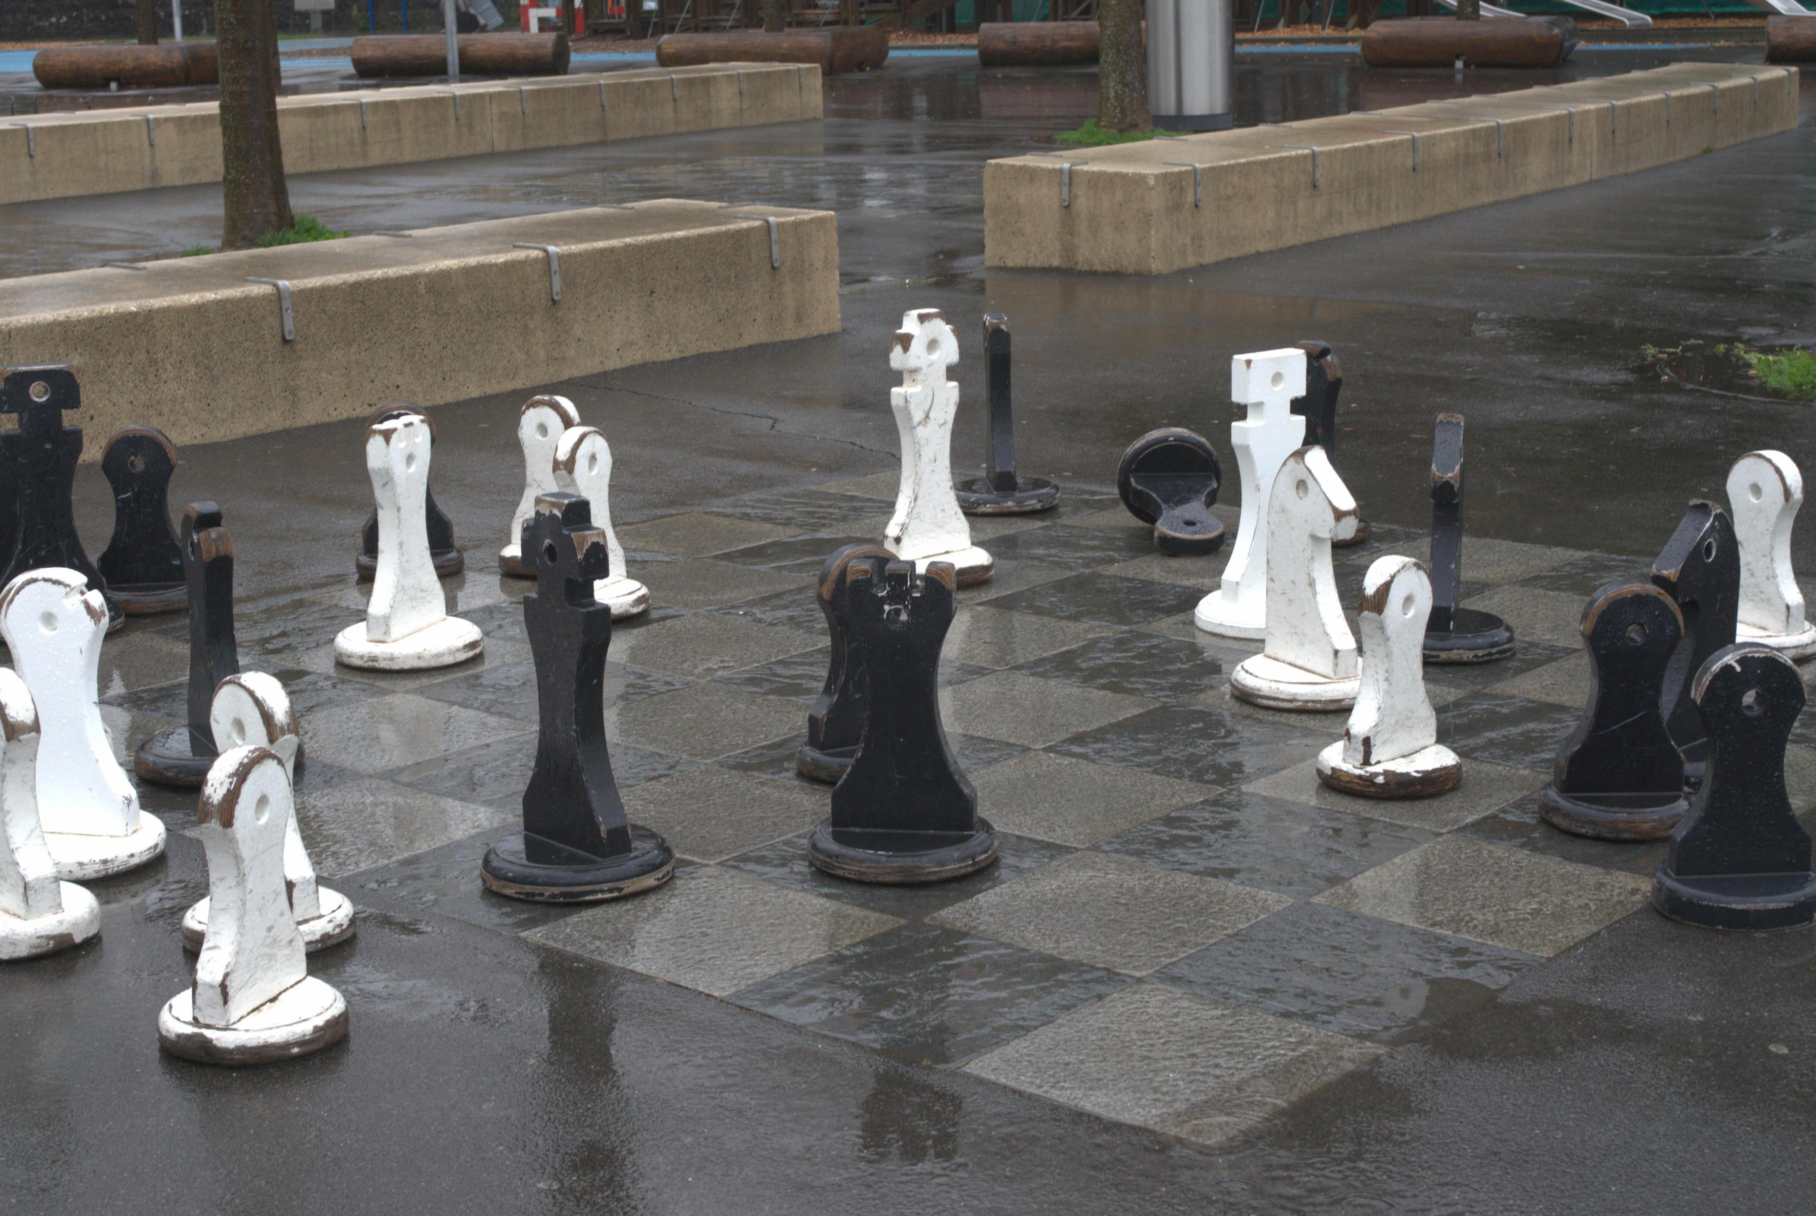
\includegraphics[width=\linewidth]{figures/digital-chess.png}
      \end{subfigure}
    \hfill
    \begin{subfigure}[t]{.24\textwidth}
        \centering
        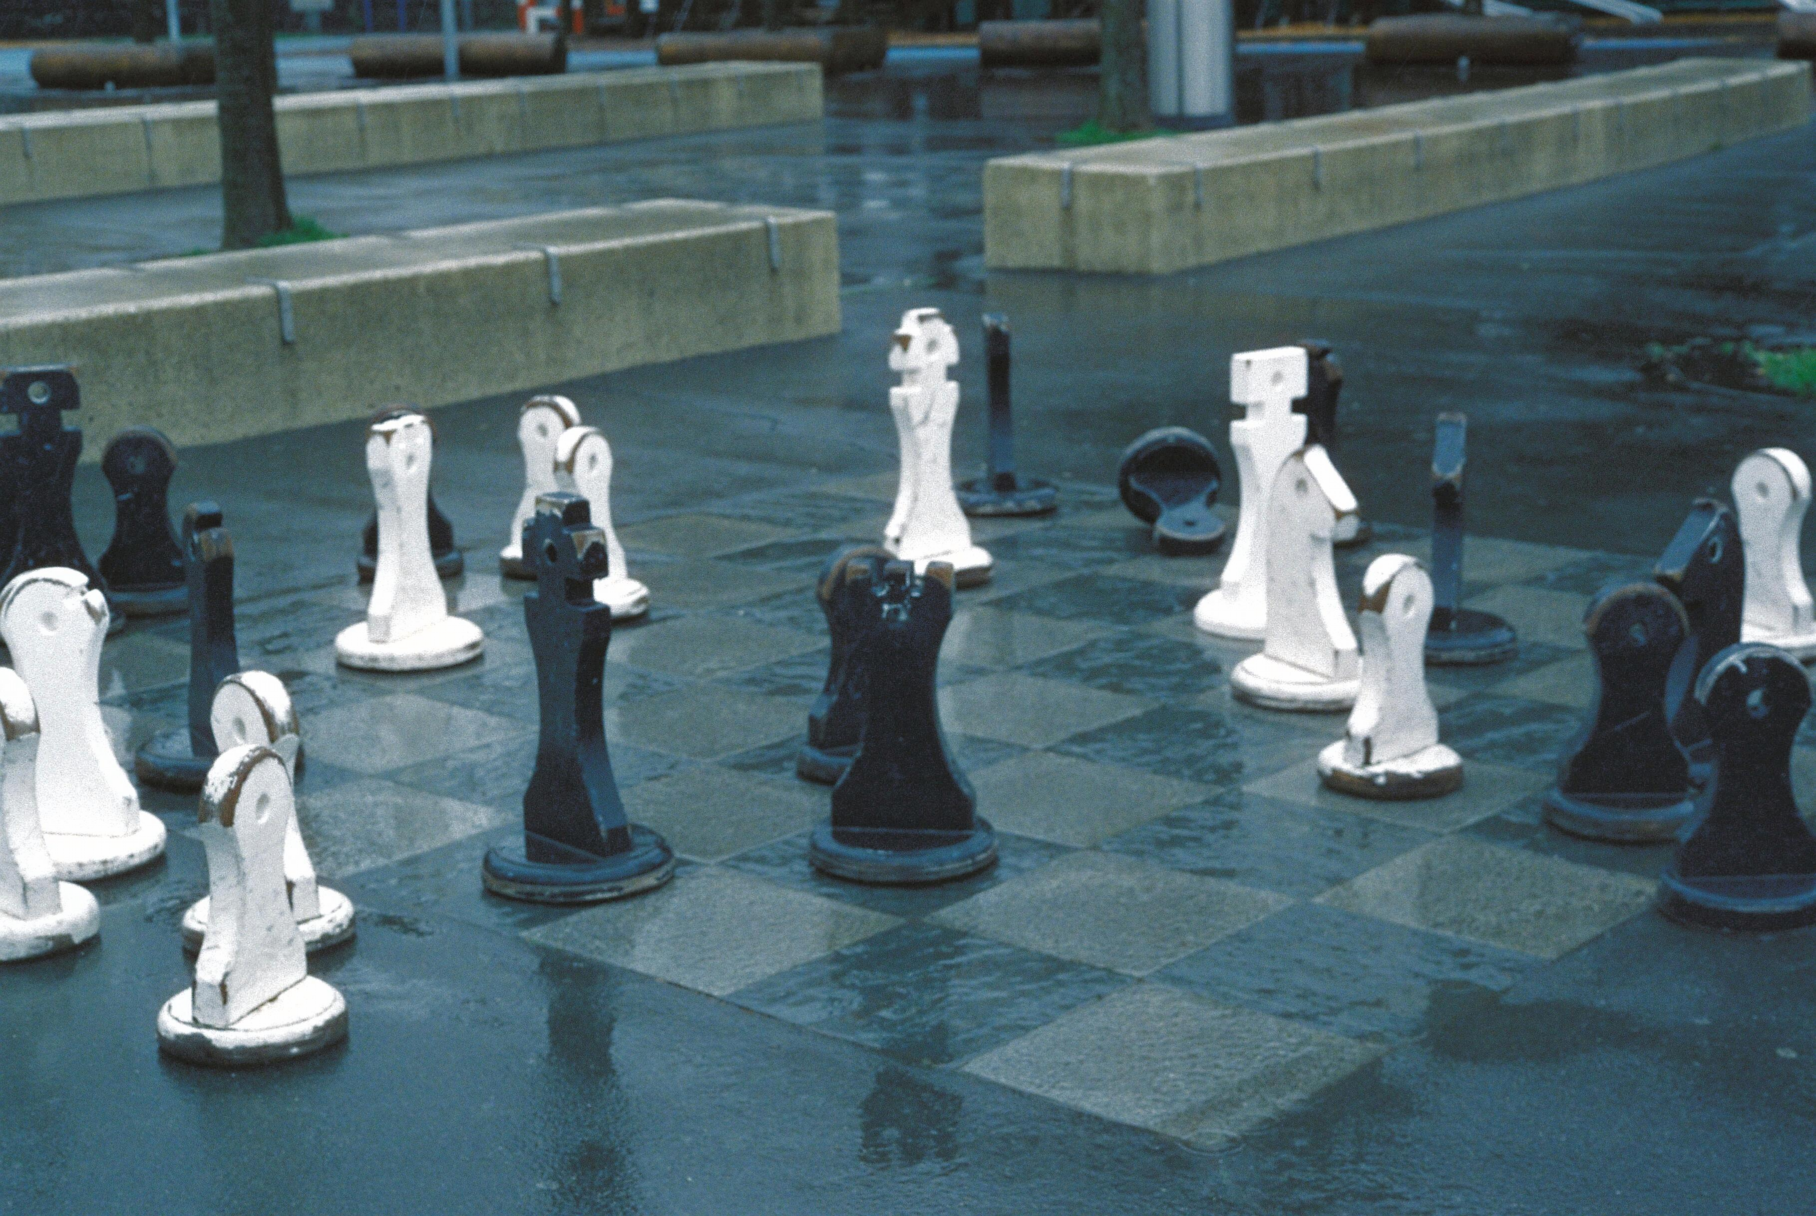
\includegraphics[width=\linewidth]{figures/film-chess.png}
      \end{subfigure}
    \hfill
    \begin{subfigure}[t]{.24\textwidth}
        \centering
        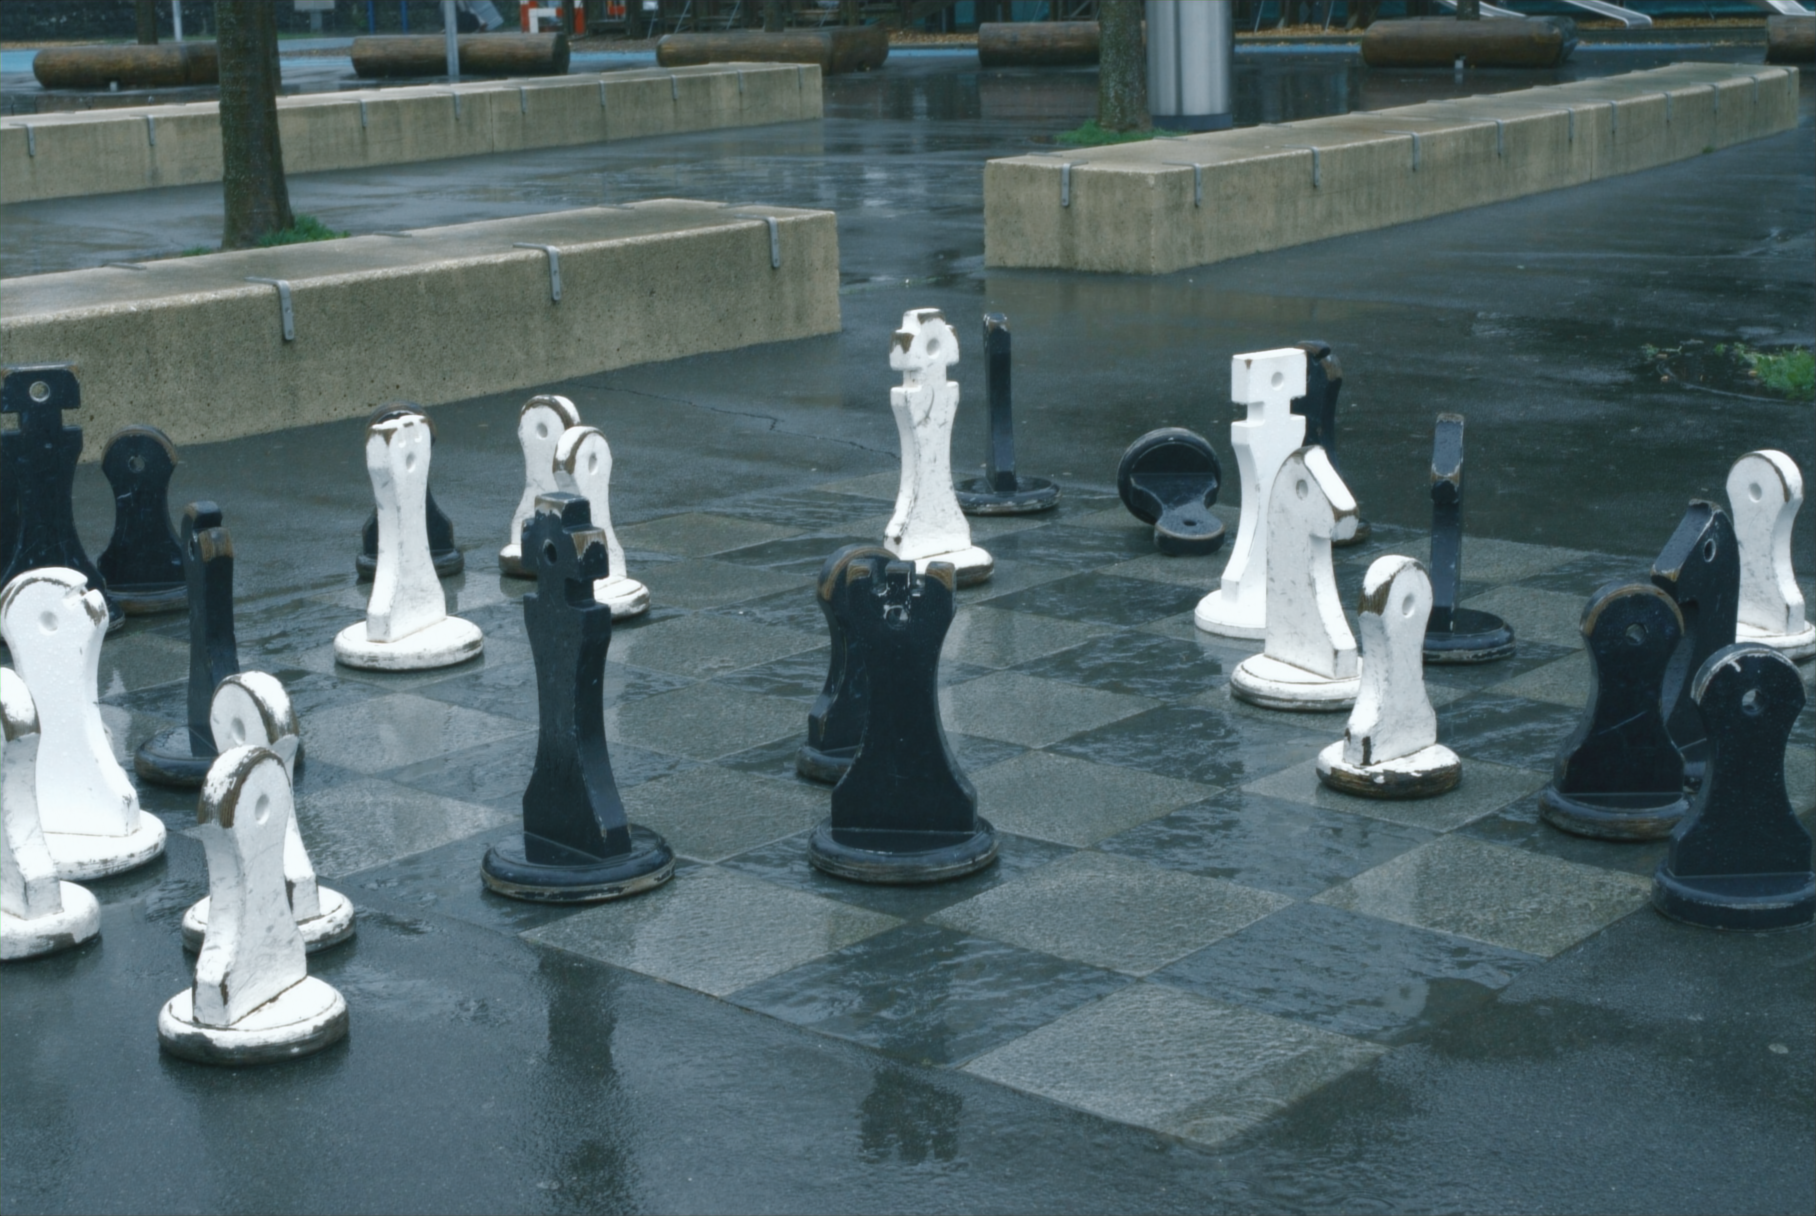
\includegraphics[width=\linewidth]{figures/mse-vgg-noise-resize-chess.png}
      \end{subfigure}
    \hfill
    \begin{subfigure}[t]{.24\textwidth}
      \centering
      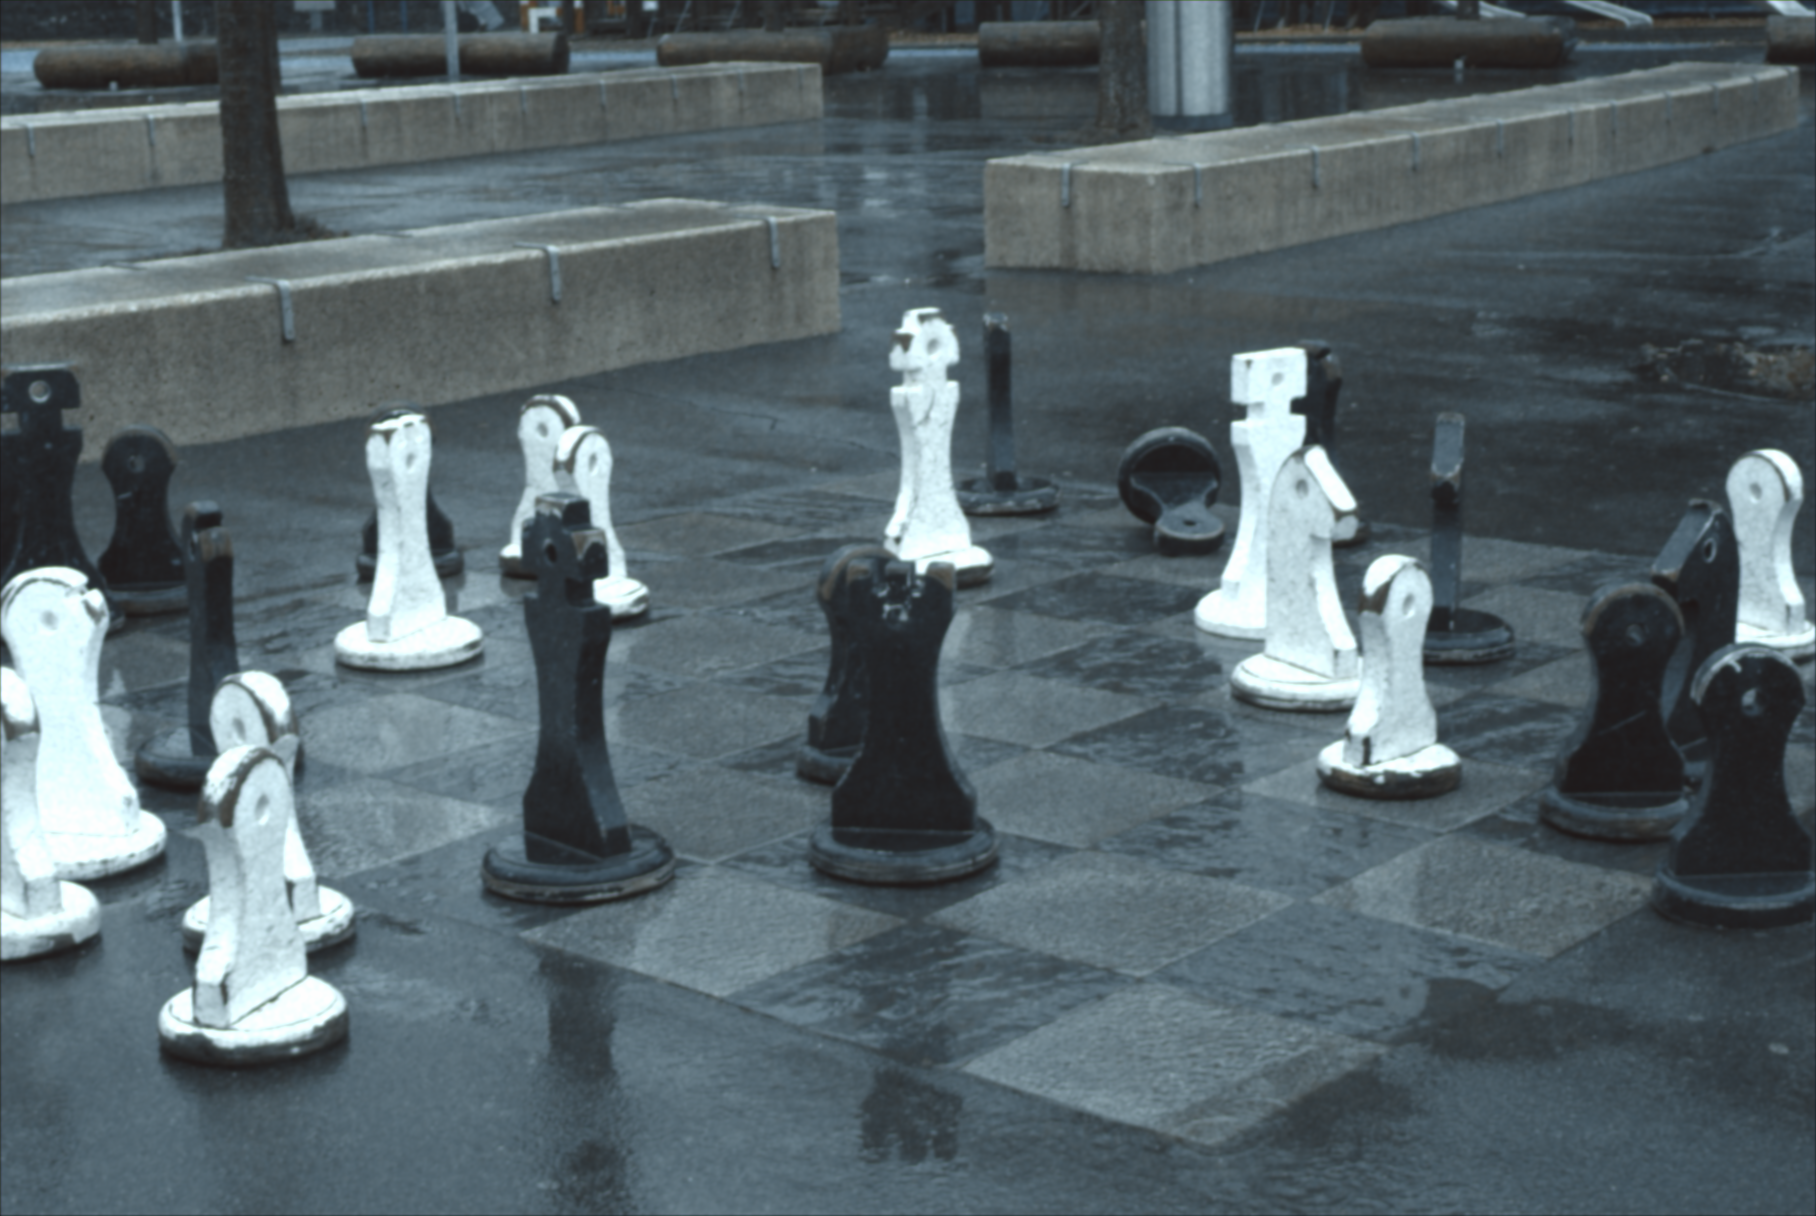
\includegraphics[width=\linewidth]{figures/color-vgg-tv-relative-chess.png}
    \end{subfigure}

    % Swisstech
    \begin{subfigure}[t]{.24\textwidth}
        \centering
        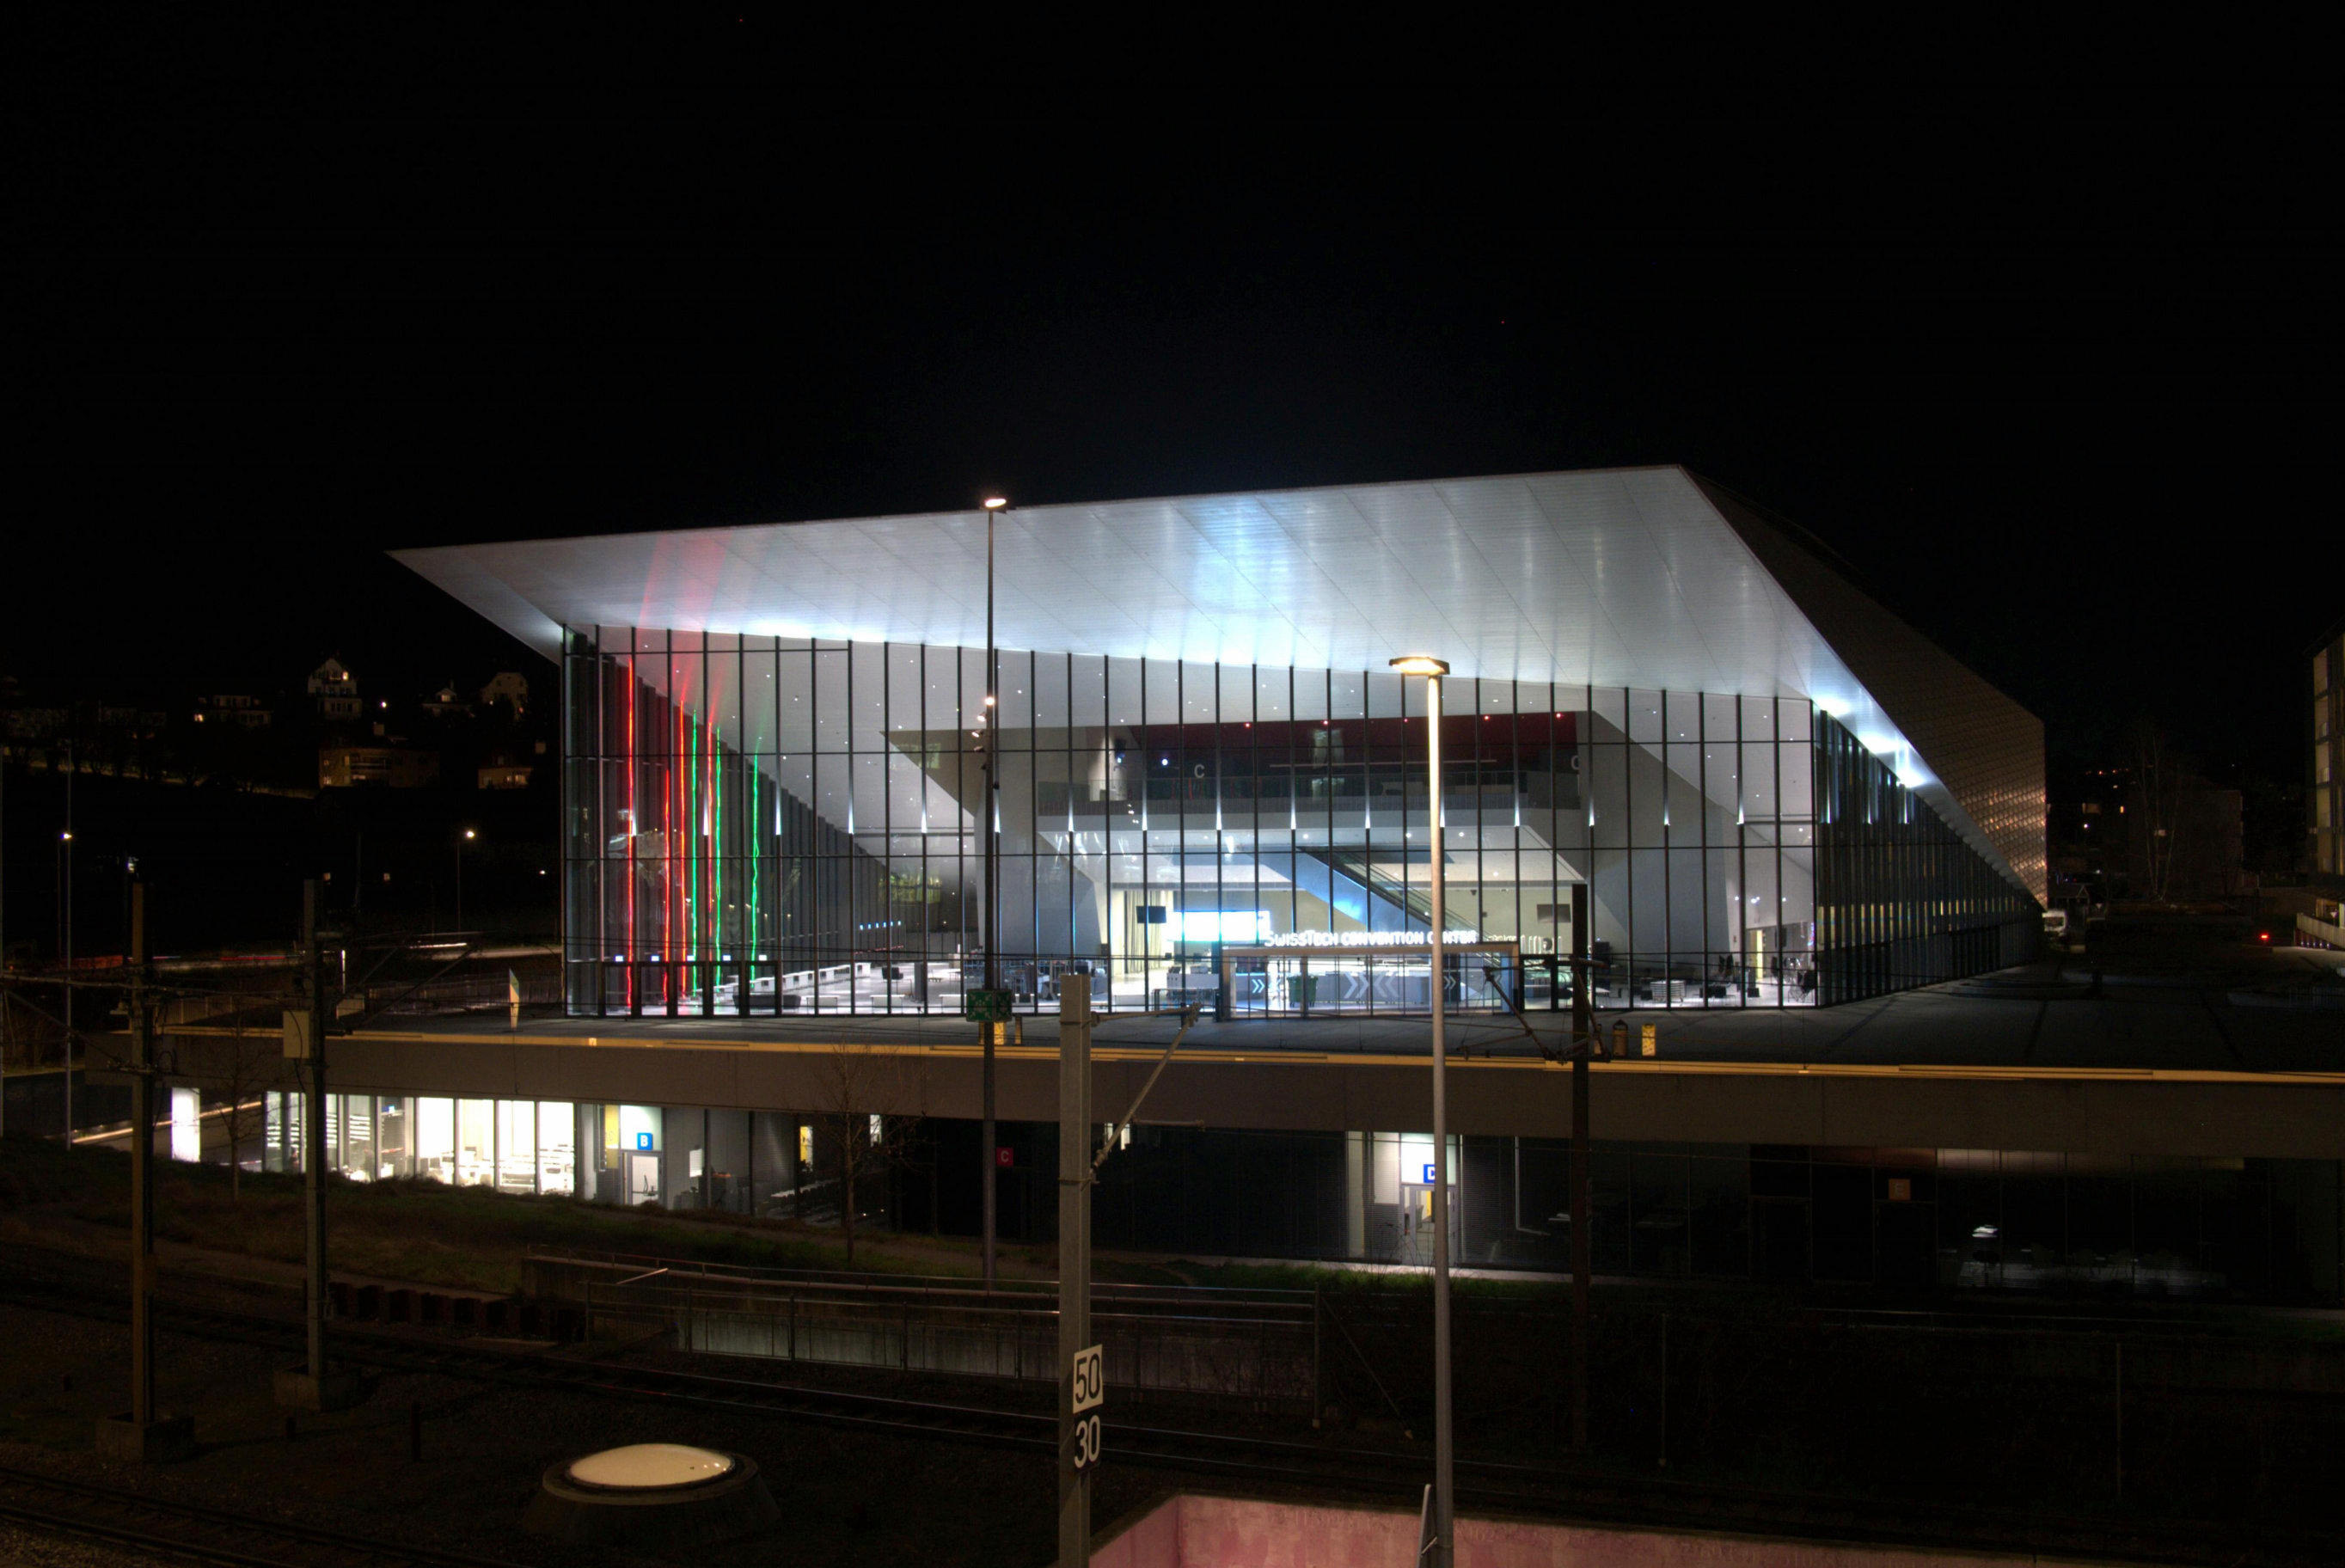
\includegraphics[width=\linewidth]{figures/digital-swisstech.png}
      \end{subfigure}
    \hfill
    \begin{subfigure}[t]{.24\textwidth}
        \centering
        \includegraphics[width=\linewidth]{figures/film-swisstech.png}
      \end{subfigure}
    \hfill
    \begin{subfigure}[t]{.24\textwidth}
        \centering
        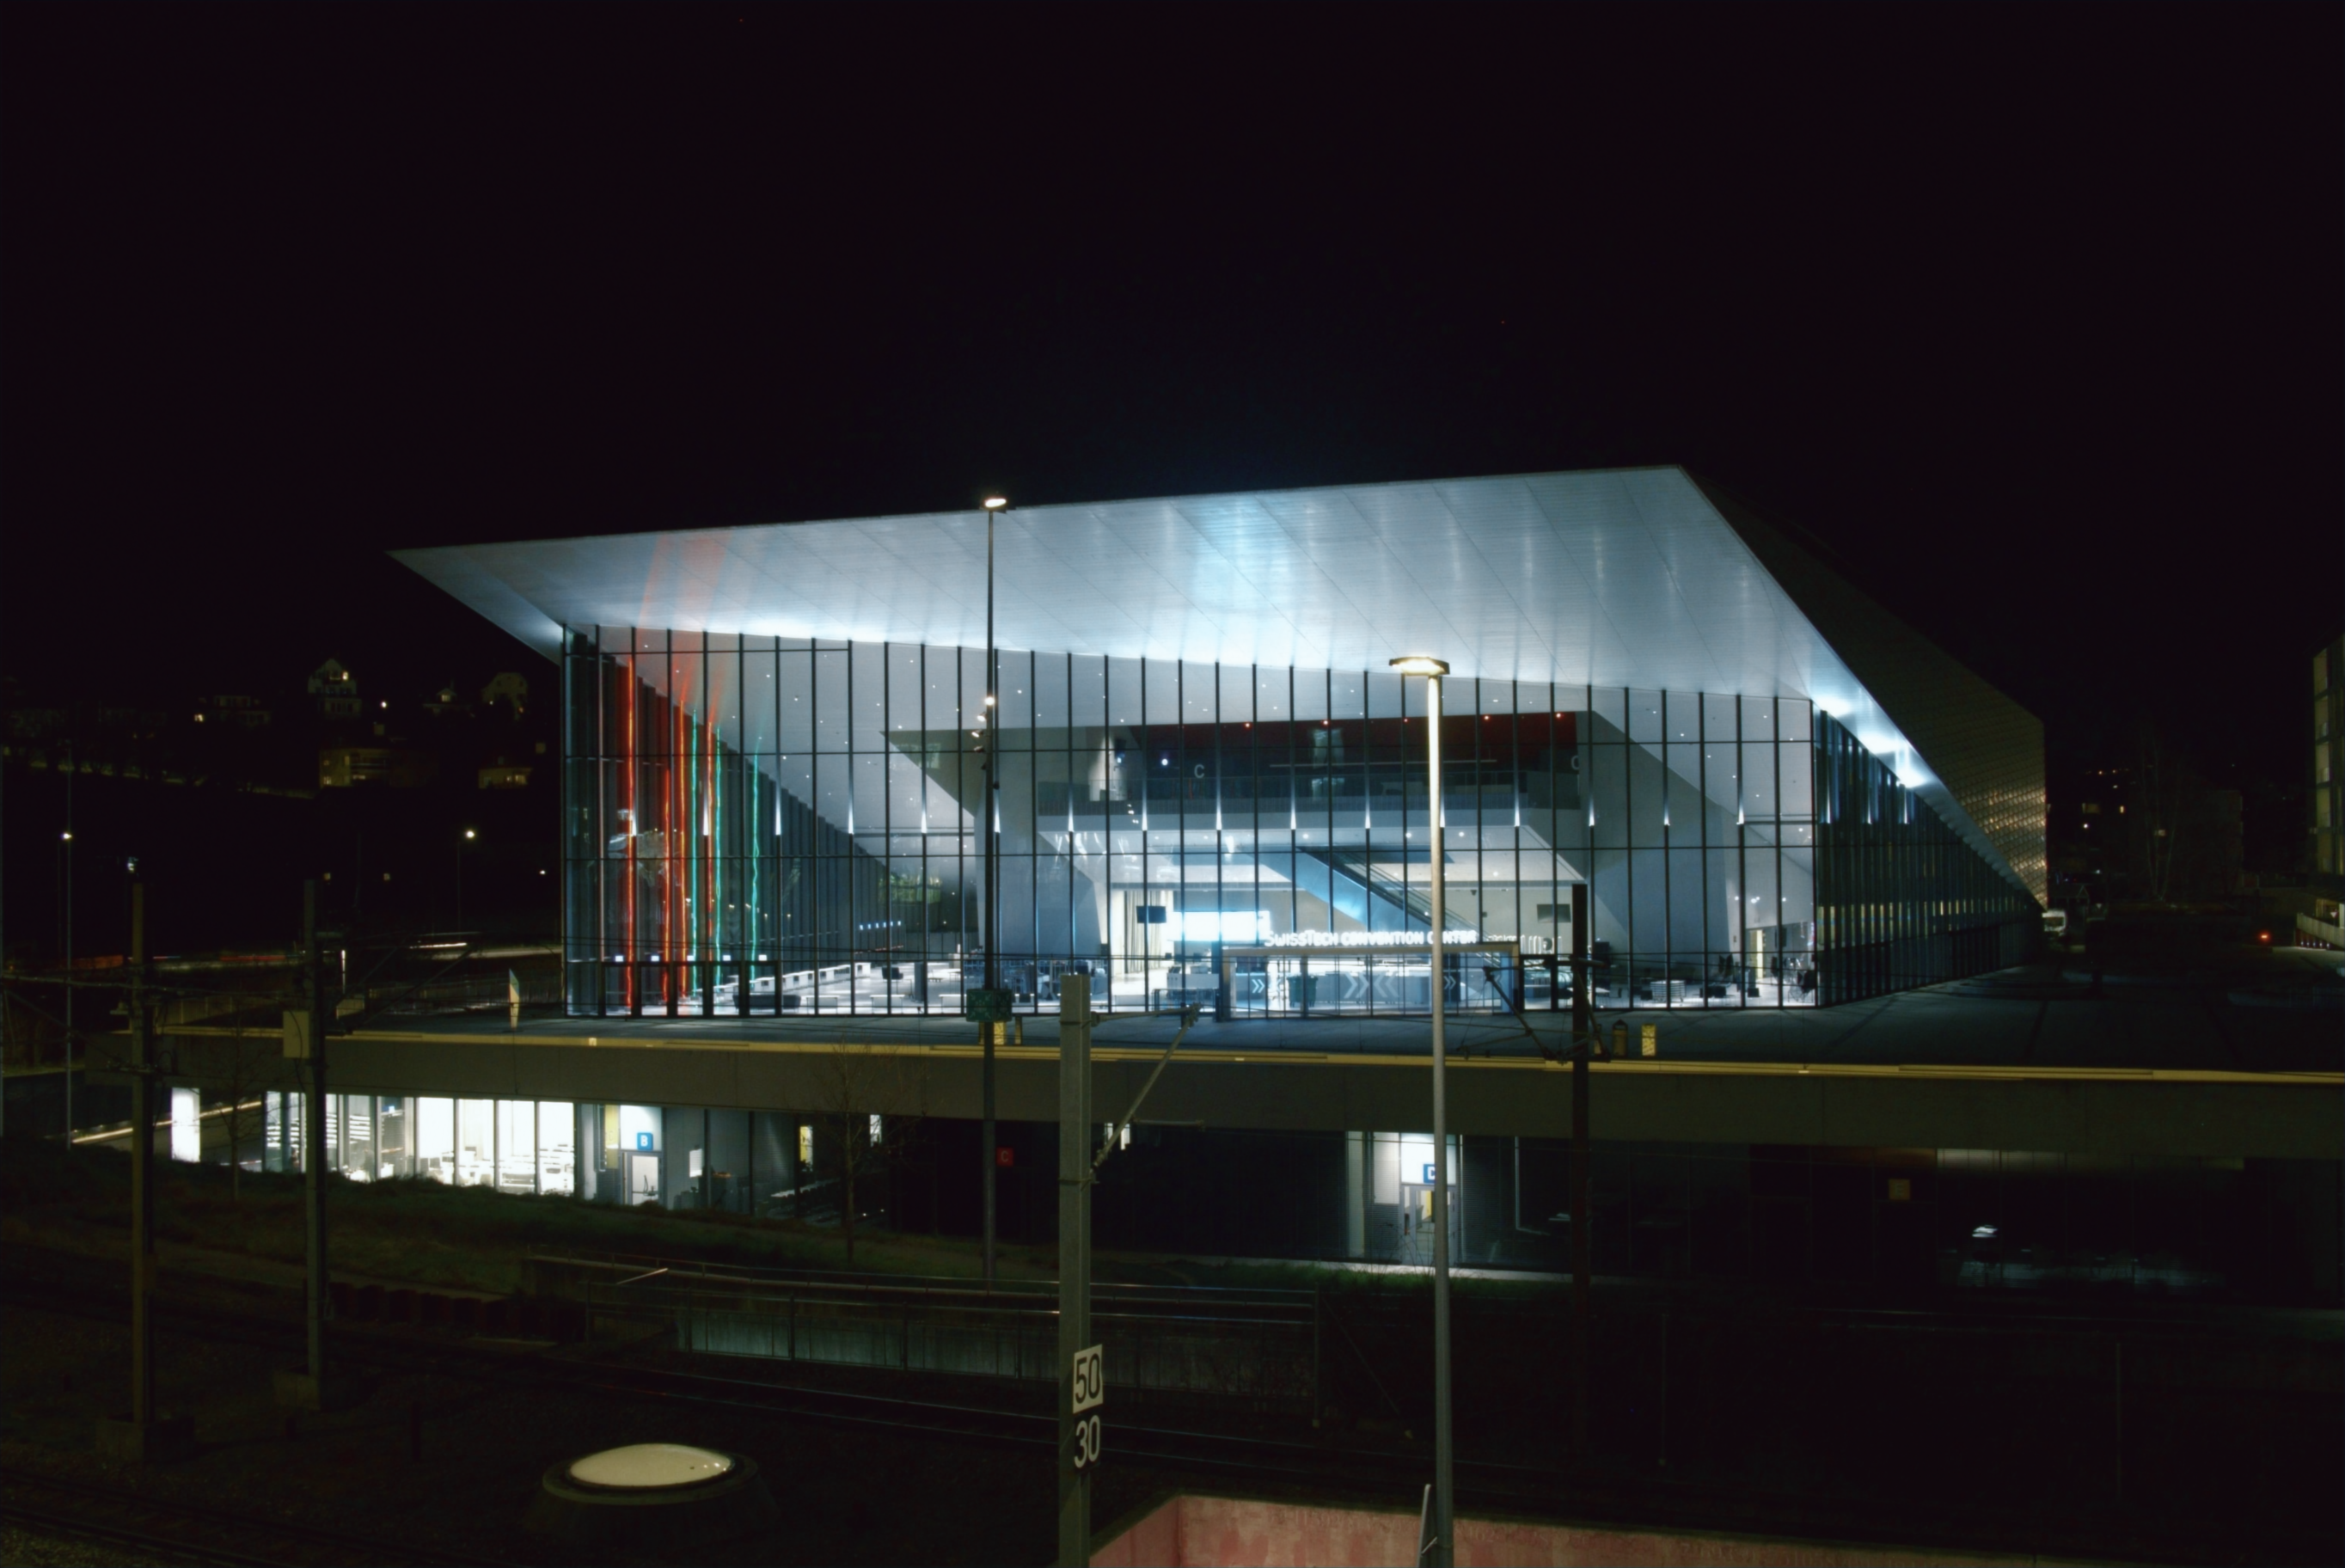
\includegraphics[width=\linewidth]{figures/mse-vgg-noise-resize-swisstech.png}
      \end{subfigure}
    \hfill
    \begin{subfigure}[t]{.24\textwidth}
      \centering
      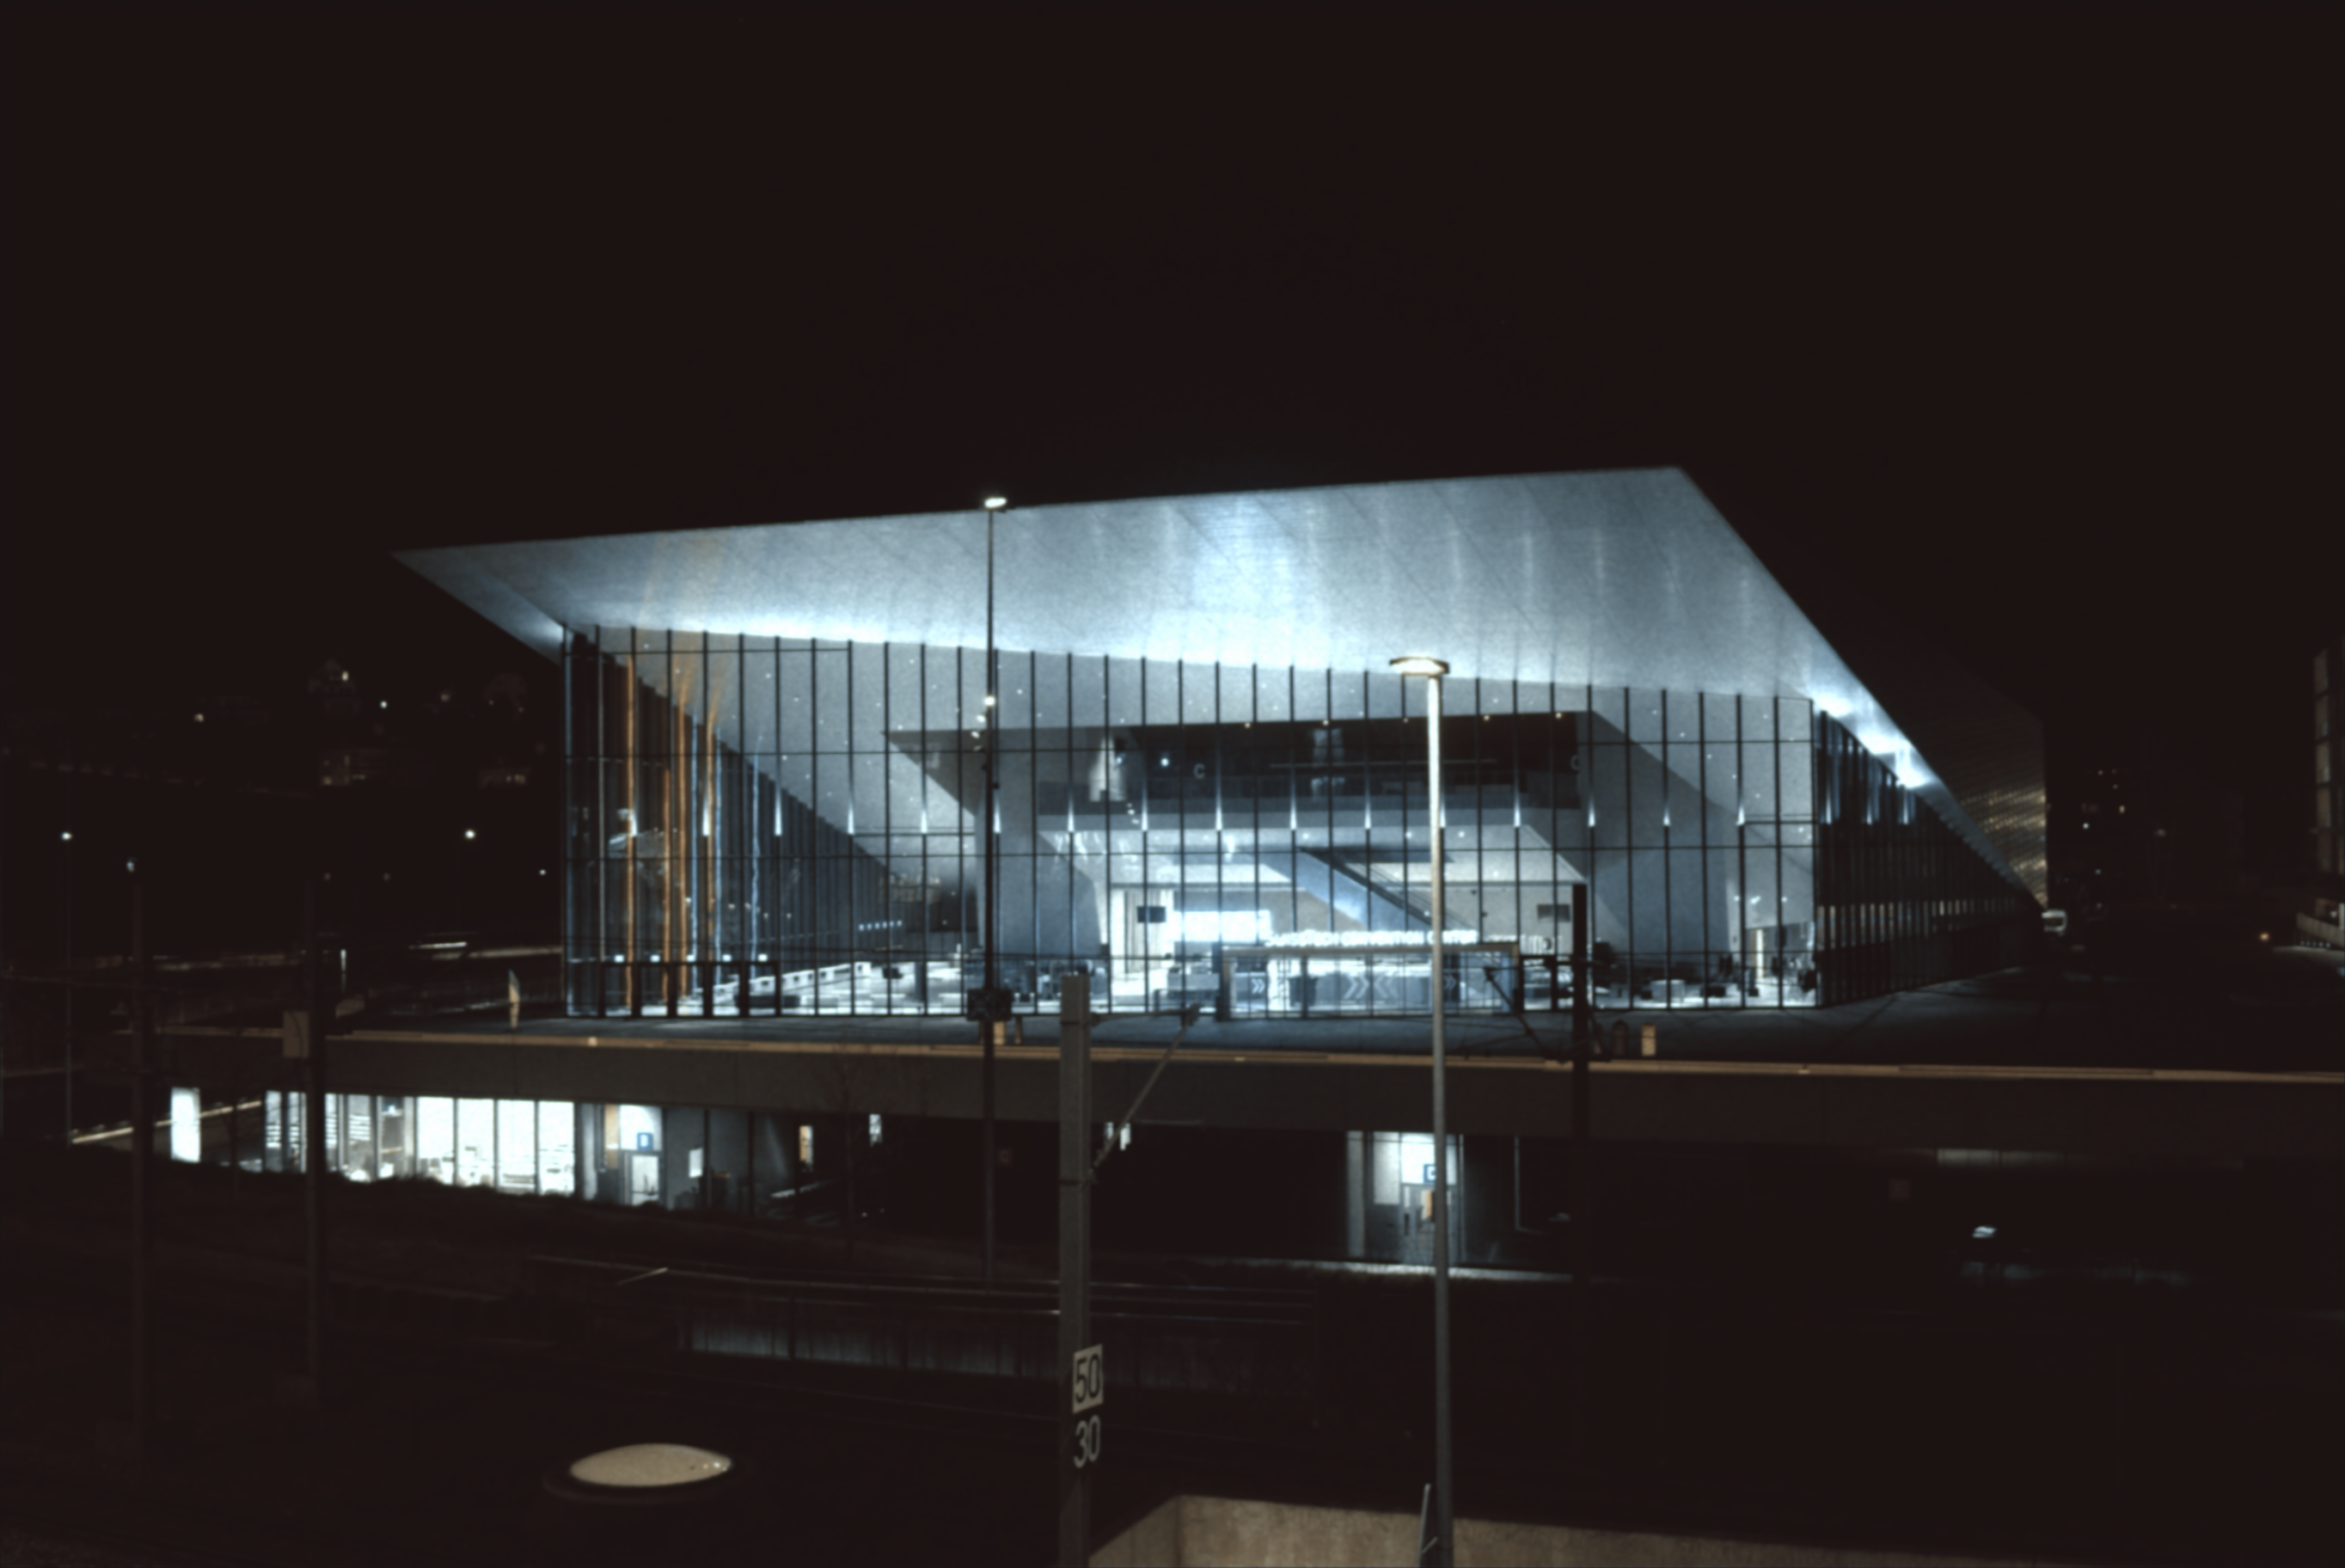
\includegraphics[width=\linewidth]{figures/color-vgg-tv-relative-swisstech.png}
    \end{subfigure}


    % Castle
    \begin{subfigure}[t]{.24\textwidth}
        \centering
        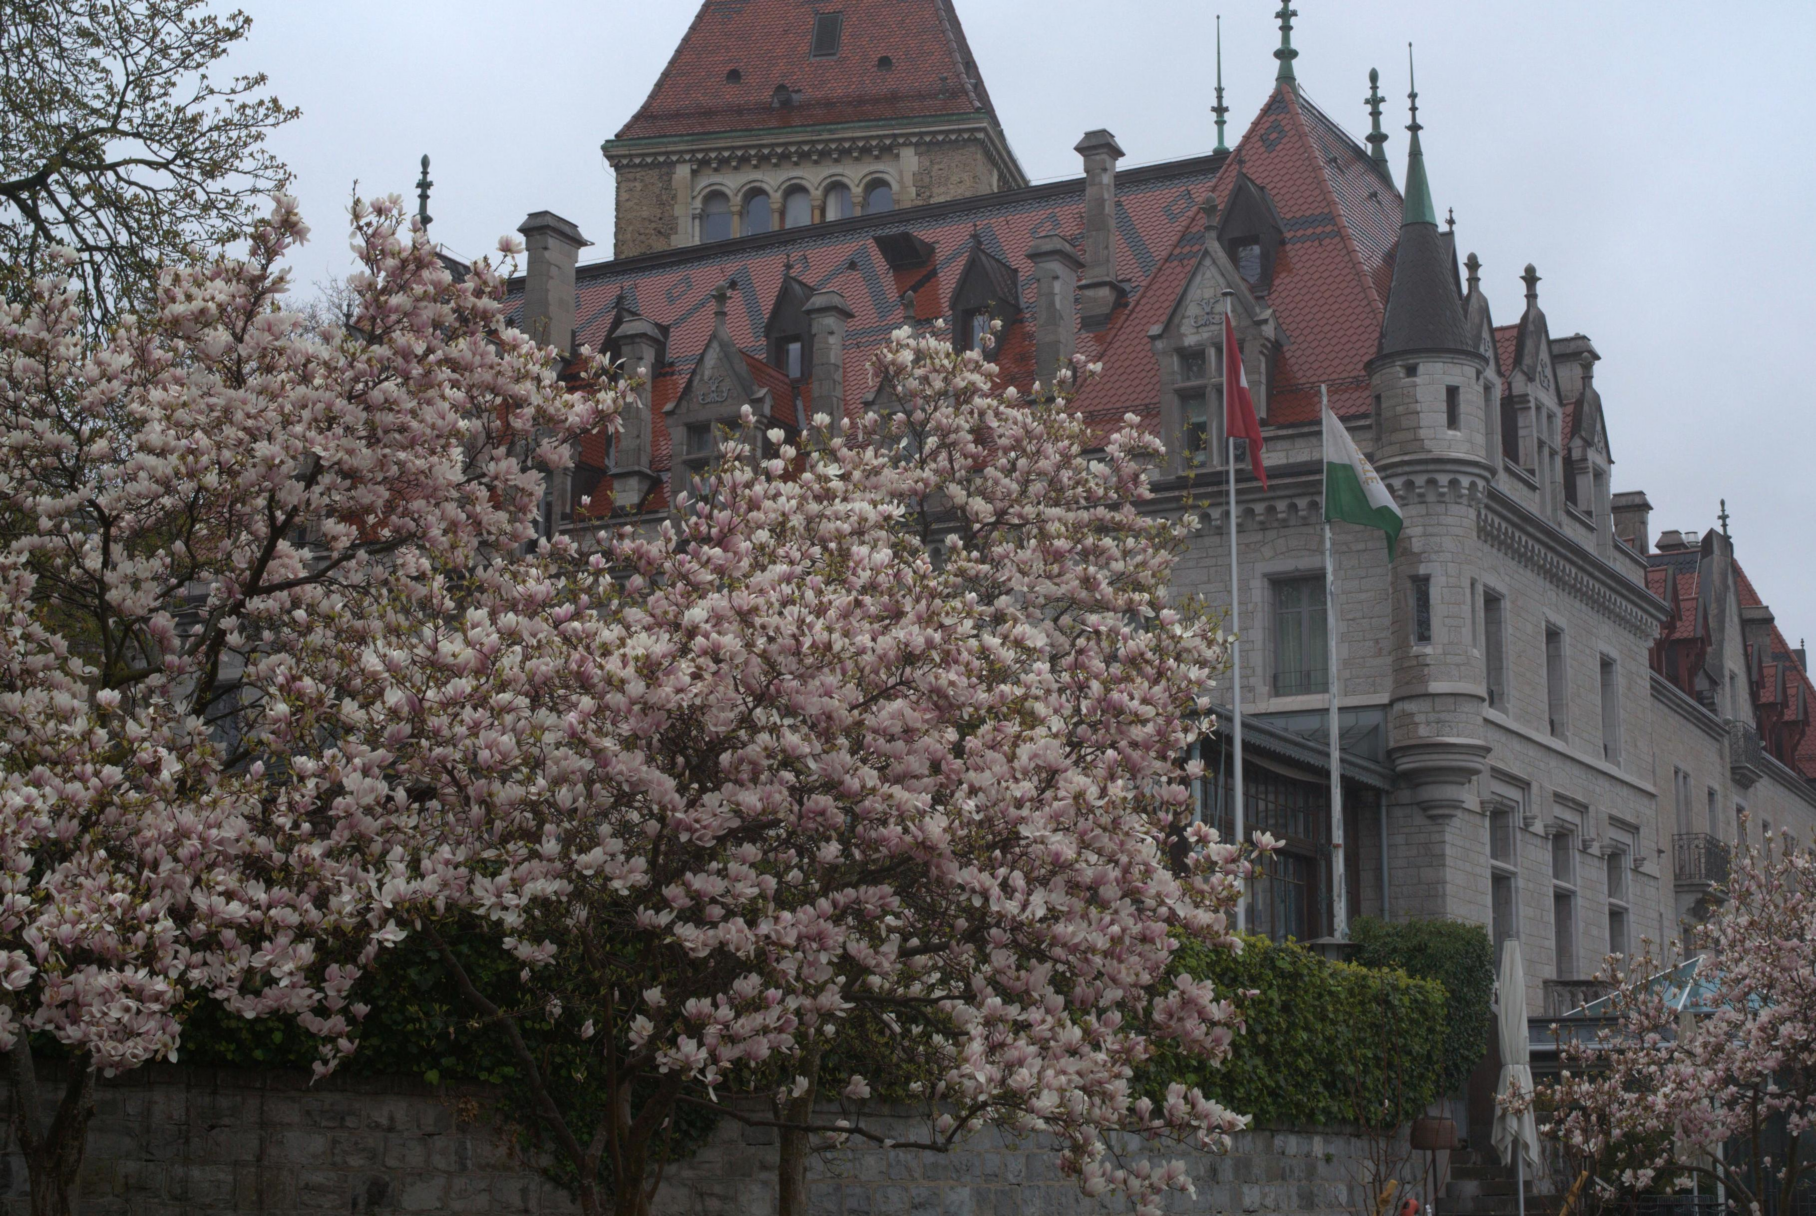
\includegraphics[width=\linewidth]{figures/digital-castle.png}
        \captionsetup{justification=centering}
        \caption{\\Digital}
      \end{subfigure}
    \hfill
    \begin{subfigure}[t]{.24\textwidth}
        \centering
        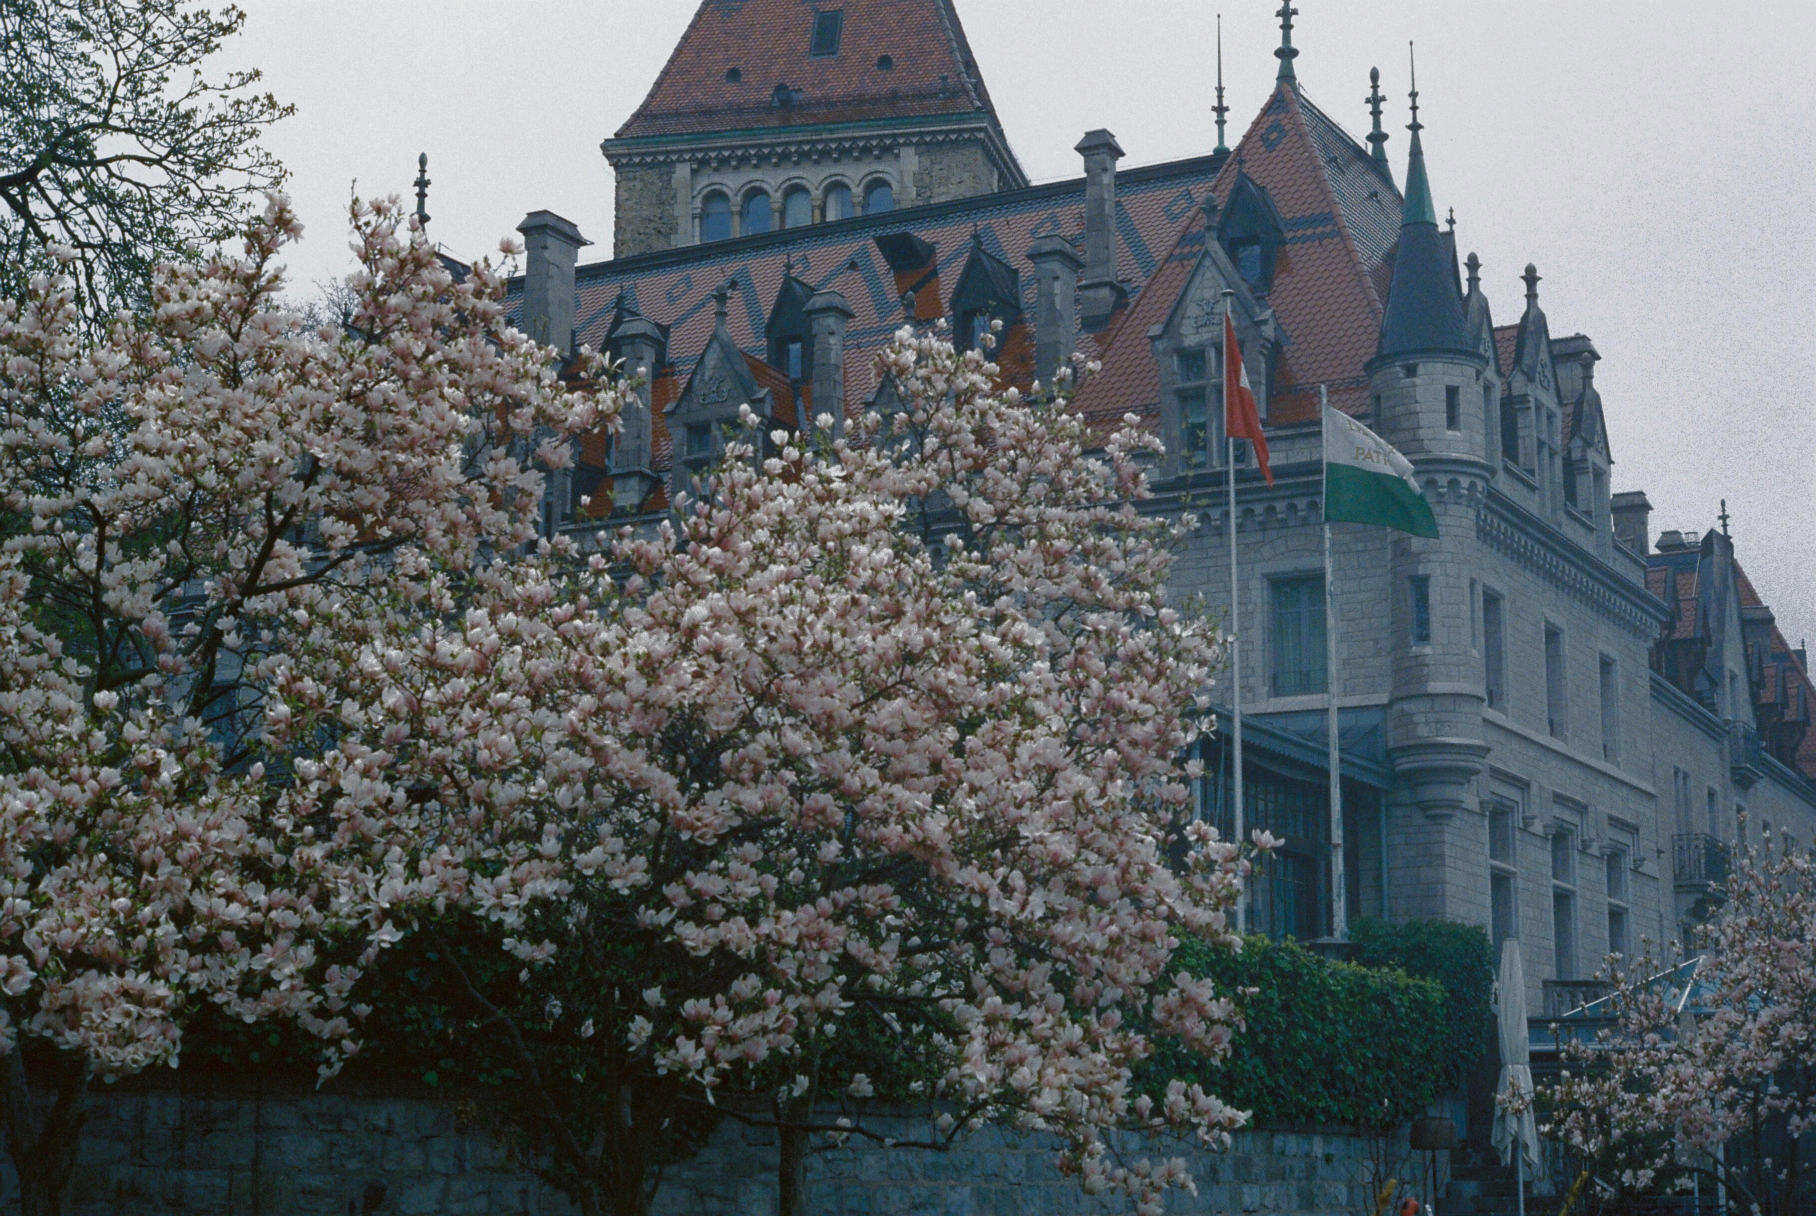
\includegraphics[width=\linewidth]{figures/film-castle.png}
        \captionsetup{justification=centering}
        \caption{\\Film}
      \end{subfigure}
    \hfill
    \begin{subfigure}[t]{.24\textwidth}
        \centering
        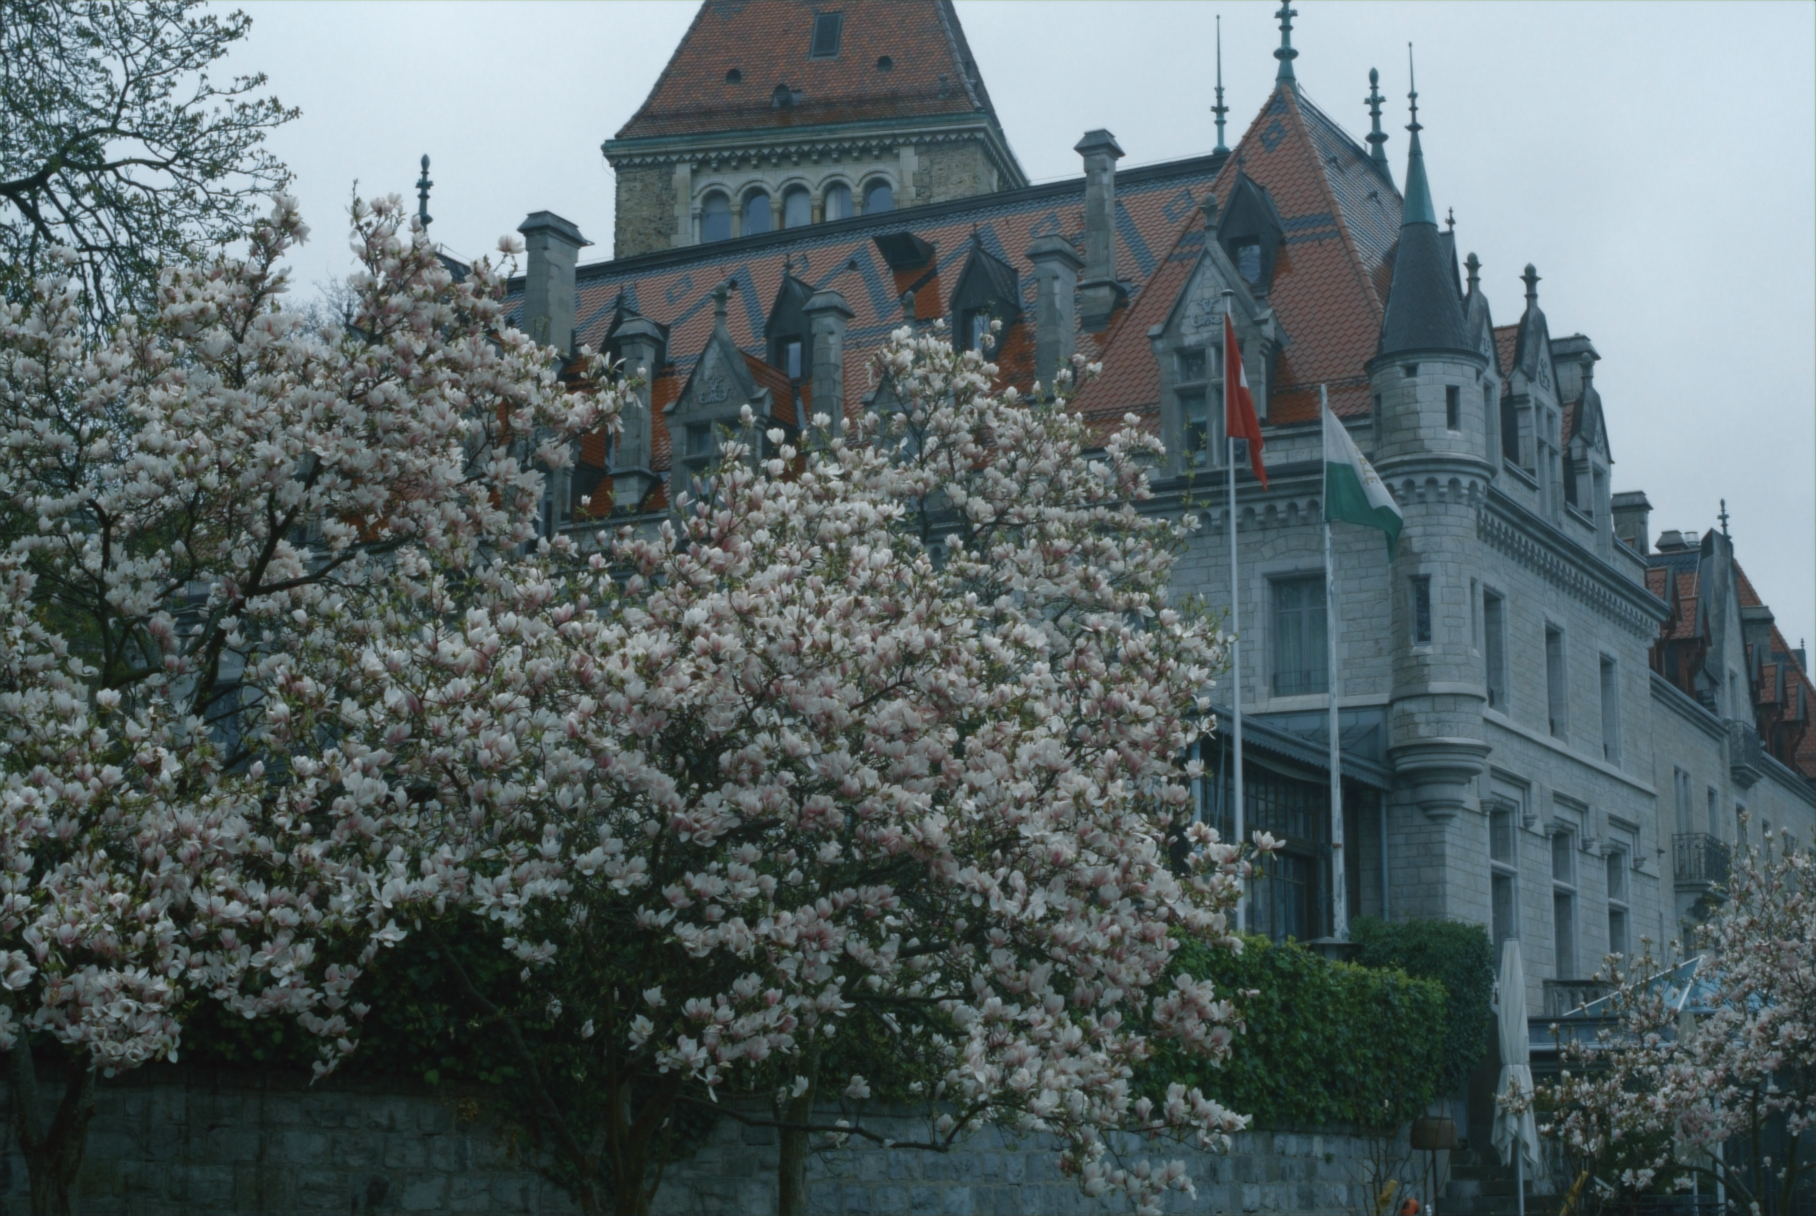
\includegraphics[width=\linewidth]{figures/mse-vgg-noise-resize-castle.png}
        \captionsetup{justification=centering}
        \caption{\\MSE/VGG}
      \end{subfigure}
    \hfill
    \begin{subfigure}[t]{.24\textwidth}
      \centering
      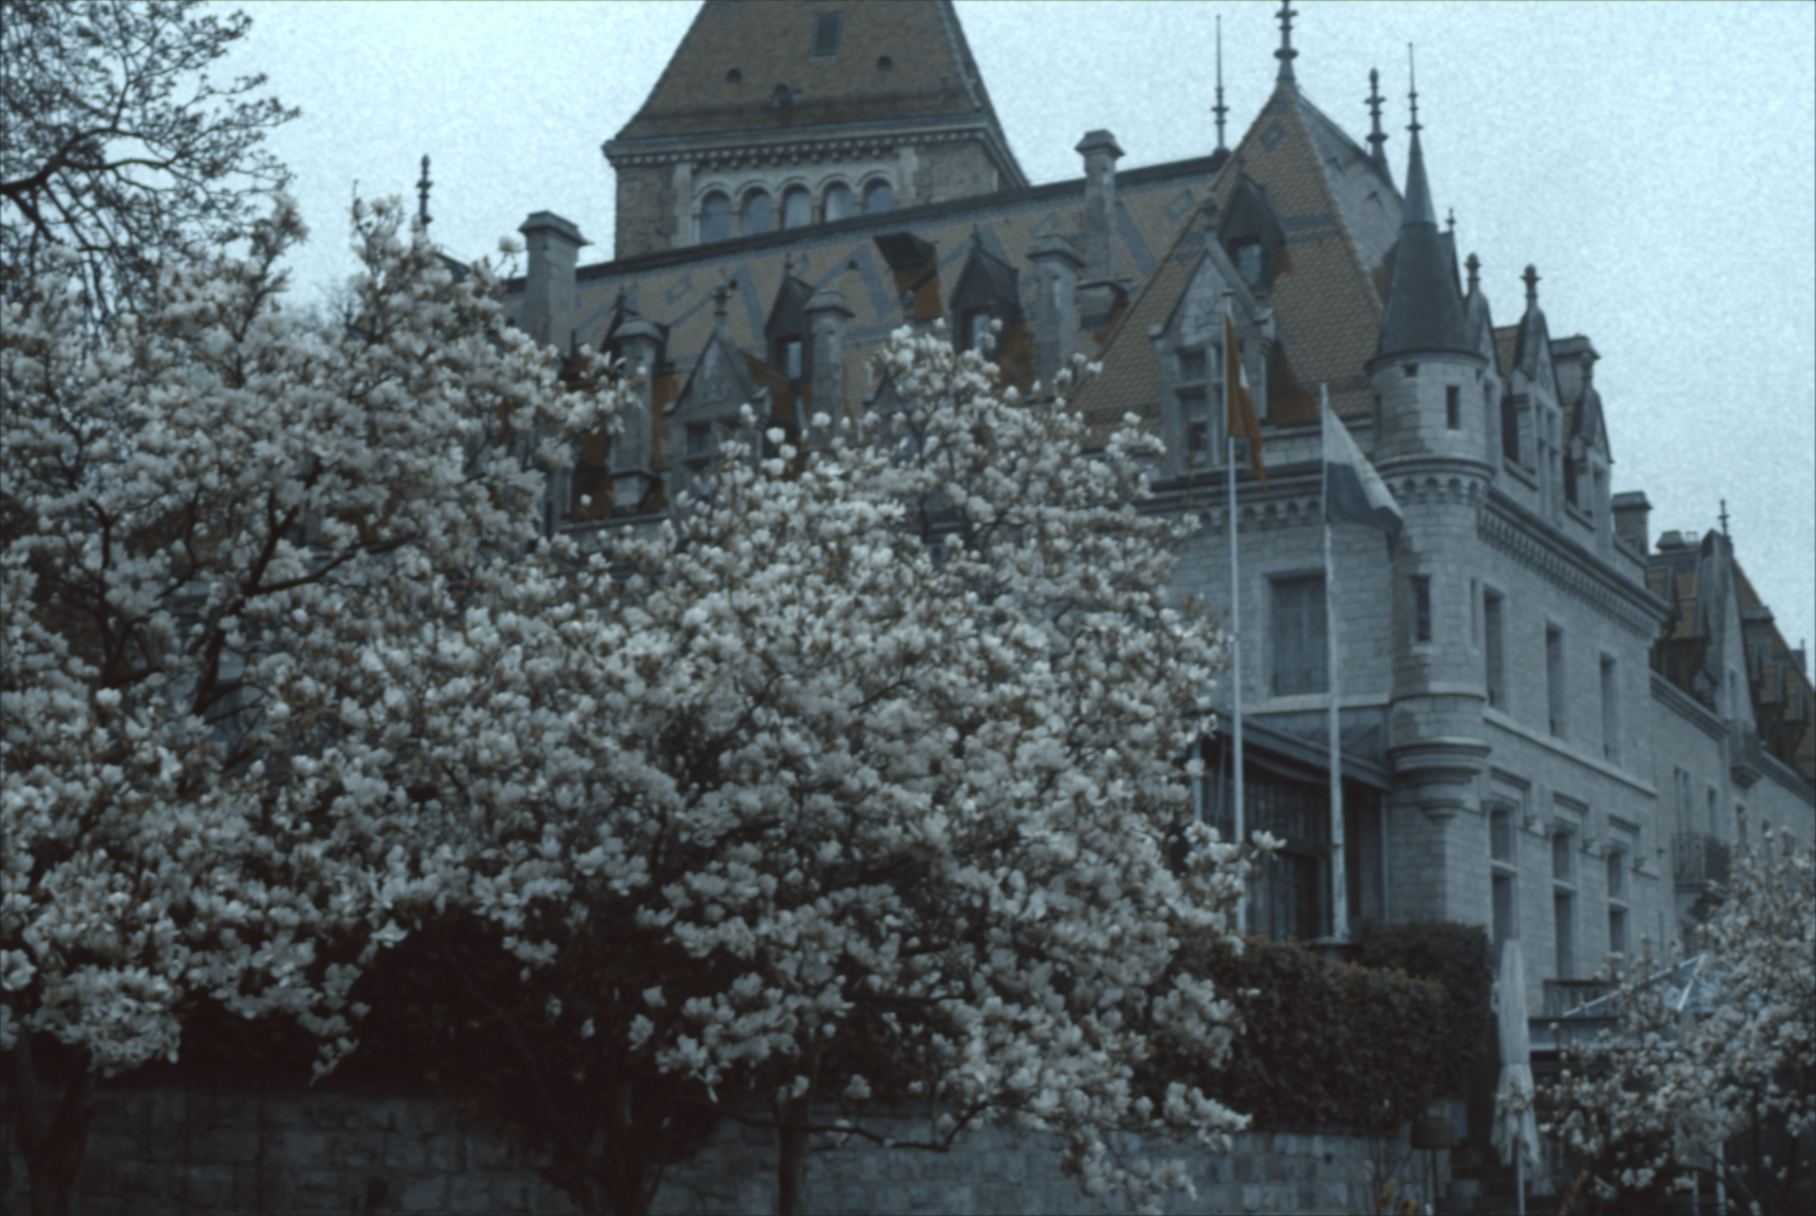
\includegraphics[width=\linewidth]{figures/color-vgg-tv-relative-castle.png}
      \captionsetup{justification=centering}
        \caption{\\Color/VGG/TV-Rel}
    \end{subfigure}

    \caption{\textbf{Full Dataset Select Samples.} Outputs from select models on the full dataset. We see that the best performing model is MSE/VGG with resizing, which produces the best colour effect. We also see that the grain effect is not as strong as in the single image experiments.}
    \label{fig:full-data-results}
\end{figure}

We continue experimenting with the presence of resizing and noise using MSE and MSE/VGG, with results found in Table \ref{tab:full-data-resize-noise}. Results indicate that once again resizing improves results, but the addition of noise has a less clear effect. The overall best performing model is MSE/VGG with resizing. Noise has little effect. However, the qualitative results tell a different story. In Figure \ref{fig:full-data-grain} we see that the model with noise produces a more visually pleasing result, with a more uniform grain effect. This is not captured by the metrics, which are more sensitive to the colour effect.

\begin{table}
    \centering
    \captionsetup{justification=centering}
    \caption{\textbf{Full Dataset Noise and Resizing.} \\ Comparison of MSE and MSE/VGG with and without noise and resizing.}
    \setlength{\tabcolsep}{0.3em}
    \begin{tabular}{lcccccc}
        \toprule
        Loss & Noise & Resize & SSIM & PSNR & LPIPS & PieAPP \\
        \midrule
        MSE/VGG & Yes & Yes & \textbf{0.64} & \textbf{22.87} & \textbf{0.27} & 1.90 \\
        MSE/VGG & No & Yes & 0.63 & 22.85 & \textbf{0.27} & \textbf{1.84} \\
        MSE/VGG & No & No & 0.58 & 20.47 & 0.50 & 3.67 \\
        \midrule
        MSE & No & Yes & \textbf{0.63} & \textbf{22.20} & \textbf{0.35} & \textbf{2.31} \\
        MSE & Yes & Yes & 0.59 & 20.87 & 0.40 & 3.29 \\
        MSE & No & No & 0.58 & 20.47 & 0.50 & 3.67 \\
        \bottomrule
    \end{tabular}
    \label{tab:full-data-resize-noise}
\end{table}

\begin{figure}
    \begin{subfigure}[t]{.19\textwidth}
        \centering
        
\includegraphics[width=\linewidth]{figures/digital-sky.png}
        \captionsetup{justification=centering}
        \caption{Digital}
      \end{subfigure}
    \hfill
    \begin{subfigure}[t]{.19\textwidth}
        \centering
        
\includegraphics[width=\linewidth]{figures/film-sky.png}
        \captionsetup{justification=centering}
        \caption{Film}
      \end{subfigure}
    \hfill
    \begin{subfigure}[t]{.19\textwidth}
        \centering
        
\includegraphics[width=\linewidth]{figures/mse-vgg-noise-resize-sky.png}
        \captionsetup{justification=centering}
        \caption{MSE/VGG}
      \end{subfigure}
    \hfill
    \begin{subfigure}[t]{.19\textwidth}
        \centering
        
\includegraphics[width=\linewidth]{figures/mse-vgg-tev-rel-sky.png}
        \captionsetup{justification=centering}
        \caption{MSE/VGG/TV-Rel}
      \end{subfigure}
      \begin{subfigure}[t]{.19\textwidth}
        \centering
        
\includegraphics[width=\linewidth]{figures/color-vgg-tv-rel-sky.png}
        \captionsetup{justification=centering}
        \caption{Color/VGG/TV-Rel}
      \end{subfigure}
    \caption{\textbf{Full Dataset Grain Comparison.} Predictions for a patch of sky from select loss functions, all with noise. Similarly to the single image experiments, the models with losses that target some noise produce a more visually pleasing result. The best visual result is produced by Color/VGG/TV-Rel although this is still far from the true grain texture.}
    \label{fig:full-data-grain}
\end{figure}

% Comparison to DSLR results

Comparing results with the related task of enhancement of mobile phone images in \cite{dslr-quality} indicates that our models have a much lower SSIM, but comparable PSNR. They achieve peak SSIM of 0.94 where we observe a peak SSIM of 0.64, whereas peak PSNR is 21.81 and 22.87 respectively. This could be due to a large range of factors such as the the quality and uniformity of the DSLR images, the difference in model architecures or the difference in losses. However, perhaps the biggest reason is the greater complexity of the film effect.

% Summary

In summary, we find that the best performing model is MSE/VGG with resizing, which produces the best metrics across the board, produces the best colour effect and often the most visually pleasing result too. The addition of noise has mixed effects but tends to help in noise production, and resizing the cropped patches during training significantly improves the learned colour transformation. The perceptual metrics better capture the output of noise by the model, and resizing allows the model to see a greater variety of areas of the image in a single patch. However, the full dataset is more complex and the models do not outperform the baseline as they did in the single image experiments. Our best model learns a good colour mapping, but the grain effect is not as strong as in the single image experiments, nor is it exactly the kind of grain observed.


% --------------------------- %

% Example 1: Exclude resized crop experiments
% \begin{table}
%     \centering
%     \caption{
%         \textbf{Full Data.}
%     }
%     \begin{tabular}{lc|cccc}
%         \toprule
%         \multicolumn{2}{c}{\textbf{Configuration}}& \multicolumn{4}{c}{\textbf{Evaluation}} \\
%         Loss & Noise & SSIM & PSNR & LPIPS & PieAPP \\
%         \midrule
%         \textbf{Baseline} & - & \textbf{0.64} {\tiny $\pm 0.09$} & \textbf{21.68} {\tiny $\pm 2.02$} & \textbf{0.26} {\tiny$\pm 0.07$} & \textbf{1.96} {\tiny $\pm 0.83$} \\
%         MAE & No & 0.59 {\tiny $\pm 0.09$} & 19.68 {\tiny $\pm 2.28$} & 0.48 {\tiny$\pm 0.08$} & 3.38 {\tiny $\pm 0.67$} \\
%         Color + VGG + TV-Rel & Yes & 0.59 {\tiny $\pm 0.11$} & 21.42 {\tiny $\pm 2.13$} & 0.41 {\tiny$\pm 0.06$} & 3.07 {\tiny $\pm 0.78$} \\
%         MSE & No & 0.58 {\tiny $\pm 0.10$} & 20.47 {\tiny $\pm 2.16$} & 0.50 {\tiny$\pm 0.08$} & 3.67 {\tiny $\pm 0.88$} \\
%         MSE + VGG & No & 0.58 {\tiny $\pm 0.10$} & 20.47 {\tiny $\pm 2.16$} & 0.50 {\tiny$\pm 0.08$} & 3.67 {\tiny $\pm 0.88$} \\
%         MSE + VGG + TV-Rel & Yes & 0.58 {\tiny $\pm 0.11$} & 20.43 {\tiny $\pm 2.29$} & 0.46 {\tiny$\pm 0.08$} & 3.54 {\tiny $\pm 0.76$} \\
%         \hline
%         \bottomrule
%     \end{tabular}
%     \label(tab:full-data-results)
% \end{table}